%% LyX 1.3 created this file.  For more info, see http://www.lyx.org/.
%% Do not edit unless you really know what you are doing.
\documentclass[english, 12pt]{article}
\usepackage{times}
%\usepackage{algorithm2e}
\usepackage{url}
\usepackage{bbm}
\usepackage[T1]{fontenc}
\usepackage[latin1]{inputenc}
\usepackage{geometry}
\geometry{verbose,letterpaper,tmargin=2.5cm,bmargin=2.5cm,lmargin=2.5cm,rmargin=2.5cm}
\usepackage{rotating}
\usepackage{color}
\usepackage{graphicx}
\usepackage{amsmath, amsthm, amssymb}
\usepackage{setspace}
\usepackage{lineno}
\usepackage{hyperref}
\usepackage{bbm}


\linenumbers
\doublespacing
%\usepackage[authoryear]{natbib}
\usepackage{natbib} \bibpunct{(}{)}{;}{author-year}{}{,} 

%Pour les rajouts
\usepackage{color}
\definecolor{trustcolor}{rgb}{0,0,1}

\usepackage{dsfont}
\usepackage[warn]{textcomp}
\usepackage{adjustbox}
\usepackage{multirow}
\usepackage{graphicx}
\graphicspath{{../figures/}}
\DeclareMathOperator*{\argmin}{\arg\!\min}

\let\tabbeg\tabular
\let\tabend\endtabular
\renewenvironment{tabular}{\begin{adjustbox}{max width=\textwidth}\tabbeg}{\tabend\end{adjustbox}}

\makeatletter

%%%%%%%%%%%%%%%%%%%%%%%%%%%%%% LyX specific LaTeX commands.
%% Bold symbol macro for standard LaTeX users
%\newcommand{\boldsymbol}[1]{\mbox{\boldmath $#1$}}

%% Because html converters don't know tabularnewline
\providecommand{\tabularnewline}{\\}

\usepackage{babel}
\makeatother


\begin{document}


\title{Predicting complex diseases: performance and robustness [OF NEW METHOD?]}
\author{Florian Priv\'e\,$^{\text{ 1,}*}$, Hugues Aschard\,$^{\text{2}}$ and Michael G.B. Blum\,$^{\text{1,}*}$}



\date{~ }
\maketitle

\noindent$^{\text{\sf 1}}$Universit\'e Grenoble Alpes, CNRS, Laboratoire TIMC-IMAG, UMR 5525, France, \\
\noindent$^{\text{\sf 2}}$Centre de Bioinformatique, Biostatistique et Biologie Int\'egrative (C3BI), Institut Pasteur, Paris, France.

\noindent$^\ast$To whom correspondence should be addressed.

\newpage
[ABSTRACT TROP LONG?]
\abstract{
Polygenic Risk Scores (PRSs) consist in combining the information across many single-nucleotide polymorphisms (SNPs) in a score reflecting the genetic risk of developing a disease. PRSs can have a major public health impact, allowing for screening campaigns to identify high-genetic risk individuals for a given disease. Yet, current PRSs are far from reaching this goal, and would have to show a high discriminative power between cases and controls in order to be of any use.

The predictive power of PRS strongly relies on the underlying technique used to include SNPs in the PRS and to estimate their relative contribution. The most commonly used method to derive PRSs is called ``Clumping+Thresholding'' (C+T). It uses only univariate genome-wide association studies (GWAS) summary statistics, which makes it very suitable and also very fast. We recently developed two R packages, bigstatsr and bigsnpr, for the analysis of large-scale genome-wide data. Package bigstatsr includes efficient functions for computing penalized linear and logistic regressions on large datasets.

We present a comprehensive comparative study of the C+T method, our penalized logistic regression and the T-Trees algorithm, which is a derivation of random forests and has shown exceptionally good predictive results in a previous study. We quickly discard the T-Trees method and show that the penalized logistic regression consistently achieves higher predictive performance while being as fast as the C+T method, whereas predictive performance of the C+T method is very sensitive to the threshold of inclusion of SNPs, depending on the disease architecture, as shown in previous studies.\\
\textbf{Contact:} \href{florian.prive@univ-grenoble-alpes.fr}{florian.prive@univ-grenoble-alpes.fr} \& \href{michael.blum@univ-grenoble-alpes.fr}{michael.blum@univ-grenoble-alpes.fr}\\
\textbf{Supplementary information:}
}

   
     



%%%%%%%%%%%%%%%%%%%%%%%%%%%%%%%%%%%%%%%%%%%%%%%%%%%%%%%%%%%%%%%%%%%%%%%%%%%%%%%%

\newpage
\section{Introduction}

Polygenic Risk Scores (PRSs) consist in combining the information across many single-nucleotide polymorphisms (SNPs) in a score reflecting the genetic risk of developing a disease. PRSs have proven to be useful for different applications, such as finding a common genetic contribution between two diseases \cite[]{purcell2009common}. 
Personalized medicine is another major application of PRSs. Personalized medicine ..will.. use PRSs in screening campaigns in order to identify high-risk individuals for a given disease. As an example of practical application, targeting screening to men at higher polygenic risk could reduce the problem of overdiagnosis and lead to a better benefit-to-harm balance in screening for prostate cancer \cite[]{pashayan2015implications}. 
Moreover, screening based on sequencing seems to make individuals positively change their health behavior, while neither causing patient anxiety nor depression \cite[]{vassy2017impact}.
Yet, PRSs would have to show a high discriminative power between cases and controls in order to be used for helping in the diagnosis of diseases. 
For example, for screening high-risk individuals and for presymptomatic diagnosis of the general population, it is suggested that the AUC must be greater than 75\% and 99\% respectively \cite[]{janssens2007impact}.

Many methods have been developed to predict disease status, or more generally any phenotype, based on SNP information.
A commonly used method, called ``P+T'' or ``C+T'' (which stands for ``Clumping and Thresholding'') -- also sometimes called genetic profiling ..or even just PRS.. -- is used to derive PRSs from results of Genome-Wide Association Studies (GWASs) \cite[]{chatterjee2013projecting,dudbridge2013power,evans2009harnessing,purcell2009common,wray2007prediction}. 
This technique only ..uses/resorts to.. summary statistics, which makes it very ..suitable.. and also very fast.
Linear Mixed-Models (LMMs) are another widely-used method in fields such as plant and animal breeding or for predicting highly heritable quantitative human phenotypes such as height \cite[]{lello2017accurate,yang2010common}. 
Yet, these models are not designed for predicting a binary trait such as a disease status and have proven not to be optimal at such ..a.. task in another comparative study \cite[]{abraham2013performance}. 
Moreover, these methods and their derivatives are often computationally demanding, both in terms of memory and time requirements, which makes them unlikely to be used for prediction on large cohorts \cite[]{golan2014effective,maier2015joint,speed2014multiblup,zhou2013polygenic}.
Finally, statistical learning methods have also been used to derive PRSs for complex human disease by jointly estimating SNP effects. Such methods include logistic regression, Support Vector Machine (SVM) and random forests \cite[]{abraham2012sparsnp,abraham2014accurate,botta2013walk,botta2014exploiting,wei2009disease}.

We recently developed two R packages, bigstatsr and bigsnpr, for efficient analysis of large-scale genome-wide data \cite[]{prive2017efficient}. Package bigstatsr includes efficient functions for computing sparse linear and logistic regressions on huge datasets. In this paper, we present a comprehensive comparative study of the C+T method, our penalized logistic regression and the T-Trees algorithm, which is a derivation of random forests and has shown exceptionally good predictive results in \cite{botta2014exploiting}. 
Note that in this comparison we do not include any LMM method for the reasons mentioned before and do not include any SVM method because it is expected to give similar results to logistic regression \cite[]{abraham2012sparsnp}.
For the C+T model, we compare different thresholds of inclusion of SNPs.
For the logistic regression, we include two novel approaches. 
First, we introduce a procedure that we call Cross-Model Selection and Averaging (CMSA) for automatically choosing the amount of regularization used (one hyper-parameter of the penalized logistic regression), which directly affects the number of SNPs included in the model. 
We also show how to use feature engineering in order to capture not only linear effects, but also recessive and dominant effects.

There have already been comparative studies on predicting human binary phenotypes based on genotype data. 
\citep{abraham2013performance} showed that penalized logistic regression and penalized SVM performed better than the standard C+T method and LMMs, for a wide-range of human diseases.
\cite{zhou2013polygenic} used simulations on real genotypes of Australian individuals to show that a hybrid of linear mixed models and sparse regression models performed better in a range of sparse to polygenic disease architectures. 
\cite{spiliopoulou2015genomic} investigated the effect of relatedness in prediction performance.
\cite{ware2017heterogeneity} evaluated best practices for using the C+T method and found out that the optimal inclusion threshold is trait-dependent. 
In this study, we particularly extend the work of \cite{abraham2013performance} by using a simulation framework similar but ..richer/more extenstive.. than the one used in \cite{zhou2013polygenic}. In order to make our comparison as comprehensive as possible, we compare different disease architectures (number, size and location of causal effects and heritability) with different model for generating liability ..scores.., one with only linear effects, and one which combines linear, dominant and ..interaction/interaction-type.. effects. First, we quickly discard T-Trees as being the ..best.. method for predicting disease status based on genotypes.
Then, we show that the penalized logistic regression consistently achieves higher predictive performance while being as fast as the C+T method, whereas predictive performance of the C+T method is very sensitive to the threshold of inclusion of SNPs, depending on the disease architecture, as shown in \cite{ware2017heterogeneity}.



%%%%%%%%%%%%%%%%%%%%%%%%%%%%%%%%%%%%%%%%%%%%%%%%%%%%%%%%%%%%%%%%%%%%%%%%%%%%%%%%

\section{Methods}

\subsection{Genotype data}

We use real genotypes of European individuals from a case/control celiac disease cohort \cite[]{dubois2010multiple}. The composition of this dataset is presented in table \ref{tab:celiac-data}.
Details of quality control and imputation for this dataset are available in \cite{prive2017efficient}.
As for simulations presented here, in order to remove the structure induced by the celiac disease status, we ..first keep only/select/restrict/retain.. controls from this cohort. 
Secondly, in order to ..alleviate.. population structure, we ..keep only.. people from the UK. Thirdly, we further subset these British people based on deviation from the robust Mahalanobis distance ..on/for.. principal components. This 3-step filtering process results in a sample of 7102 individuals with minimal population structure (see supplementary notebook ``preprocessing''). 
Note that we decided to ..alleviate.. population structure because it can affect the predictive performance of methods, which we will investigate in another study.


\subsection{Simulations of phenotypes} \label{sec:simus}

In order to simulate phenotypes, we use the Liability Threshold Model (LTM) with a prevalence of 30\% [CITATION?]. We vary different parameters: the number of chromosomes used (either all 22 chromosomes or only chromosome 6), the size of the training set ($\{1000, 2000, \dots, 6000\}$), the number of causal variants and their location (30, 300 or 3000 anywhere on the genome or 30 only in the HLA region), the heritability (50\% or 80\%), the distribution of effects associated with causal SNPs (Normal or Laplace), and the model used to generate the genetic ..part/component/term.. of the phenotypes (a ``simple'' model with only linear effects, and a ``fancy'' model which combines linear, dominant and ..interaction/interaction-type.. effects).
For the ``simple'' model, we compute $$y_i = \sum_{j\in E_\text{causal}} w_j \cdot \widetilde{G_{i,j}}$$ where $w_j$ are weights (generated with a Gaussian or a Laplace distribution), $G_{i,j}$ is the allele count of individual $i$ for SNP $j$ and $\widetilde{G_{i,j}}$ corresponds to its standardized version (zero mean and unit variance for all SNPs). 
For the ``fancy'' model, we separate the causal SNPs in three equal sets $E_\text{causal}^{(1)}$, $E_\text{causal}^{(2)}$ 
and $E_\text{causal}^{(3)}$ ($E_\text{causal}^{(3)}$ is further separated in two equal sets, $E_\text{causal}^{(3.1)}$ and $E_\text{causal}^{(3.2)}$). 
We then compute $$y_i = \underbrace{\sum_{j\in E_\text{causal}^{(1)}} w_j \cdot \widetilde{G_{i,j}}}_\text{linear} + \underbrace{\sum_{j\in E_\text{causal}^{(2)}} w_j \cdot \widetilde{D_{i,j}}}_\text{dominant} + \underbrace{\sum_{\substack{k=1 \\ j_1=e_k^{(3.1)} \\ j_2=e_k^{(3.2)}}}^{k=\left|E_\text{causal}^{(3.1)}\right|} w_{j_1} \cdot \widetilde{G_{i,j_1} G_{i,j_2}}}_\text{interaction}$$ 
where $D_{i,j} = \mathds{1}\left\{G_{i,j} \neq 0\right\}$ and $E_\text{causal}^{(q)}=\left\{e_k^{(q)},~k \in \left\{1, \ldots, \left|E_\text{causal}^{(q)}\right|\right\}\right\}$. 
Note that for the interaction part of the model, we scale interactions, not the raw allele counts, so that corresponding SNPs still ..display/have.. a marginal effect. 
For both models, the ..$y_i$/values of $y_i$.. are then standardized to make sure they have a variance exactly equal to the desired heritability $h^2$ and we further add some environmental noise $\epsilon_i$ to $y_i$, where $\epsilon \sim N(0, 1 - h^2)$.


We ..make/construct/design/implement/work with.. 3 different simulation scenarios, summarized in table \ref{tab:simus}. 
Scenario \textnumero1 uses the whole dataset (all 22 autosomal chromosomes) and a training set of size 6000. It compares all methods described in section \ref{sec:methods} ..on/for/along/in relation to.. all other combinations of parameters in 100 simulations (i.e.\ 5 times more than in \cite{zhou2013polygenic}). Note that the T-Trees method is compared on only 5 simulations and an heritability of 80\%, which aims at quickly discarding this method that can require more than one hour of computation for a single simulation only. 
Scenario \textnumero2 consists of 100 simulations comparing the ``logit-simple'' and the C+T methods on a dataset composed of chromosome 6 only. Reducing the number of SNPs aims at increasing the polygenicity of the simulated models and at ..virtually/artificially.. increasing the sample size [REF? DUDBRIDGE?]. For this scenario, we use only the additive (``simple'') model, but continue to compare all previous variations of the other parameters.
Finally, scenario \textnumero3 reuses the whole dataset but this time varying the size of the training set in order to assess how the sample size affects predictive performance of the PRS and the ``logit-simple'' methods. 100 simulations are run using 300 causal SNPs anywhere on the genome. 


\subsection{Predictive performance measures}\label{sec:auc}

In this study, we use two different measures of predictive accuracy. 
First, we use the Area Under the Receiver Operating Characteristic (ROC) Curve (AUC) \cite[]{fawcett2006introduction,hanley1982meaning,lusted1971signal}. In the case of our study, the AUC is the probability that a PRS of a case is greater than the PRS of a control.
This measure indicates the extent to which we can distinguish between cases and controls using PRSs.
As a second measure, the partial AUC for specificities between 90\% and 100\% is also reported \cite[]{dodd2003partial,mcclish1989analyzing}. This measure is similar to the AUC, but focuses on high specificities (i.e.\ discarding most of the healthy population as being diseased), which is often the most useful part of the ROC curve in clinical settings. 

%Note that we also report the timing of the main computations and the number of SNPs used in the predictions.

\subsection{Methods compared} \label{sec:methods}

In this study, we compare three different types of methods: the C+T method, the T-Trees method and a penalized logistic regression.

The C+T (Clumping + Thresholding) method directly derives a Polygenic Risk Score (PRS) from the results of a Genome-Wide Associations Studies (GWAS), referred to as summary statistics.
For the C+T method, a coefficient of regression is learned independently for each SNP along with a corresponding p-value (the GWAS part). 
The SNPs are first clumped (C) so that there remain only loci that are weakly correlated with one another. 
Then, thresholding (T) consists in removing SNPs that are within a certain level of significance (p-value threshold to be determined). 
Finally, a PRS is defined as the sum of allele counts of the remaining SNPs weighted by the corresponding effect coefficients: $$S_i(T, E_\text{clumping}) = \sum_{j \in E_\text{clumping}} \mathds{1}\{p_j < T\} \cdot \beta_j \cdot G_{i,j}$$ where $\beta_j$ ($p_j$) are the effect sizes (p-values) learned from the GWAS and $T$ is a threshold on p-values to be determined. In this study, we report scores for a clumping threshold at $r^2 > 0.2$ within regions of 500kb. 

For the C+T method, we report three different scores of prediction: one including all the SNPs (remaining after clumping), one including only SNPs that have a p-value under the GWAS threshold of significance ($p < 5 \cdot 10^{-8}$), and one that maximizes the AUC for these two thresholds and a sequence of 100 values of thresholds ranging from $10^{-0.1}$ to $10^{-100}$ and equally spaced on the log-log-scale (Table \ref{tab:thr}). 
Note that, normally, this optimal threshold would have to be learned based on the training set only in order to prevent from over-fitting the data. We consider this reported maximum AUC as an upper bound of the AUC for the C+T method.
We call these three reported scores respectively ``PRS-all'', ``PRS-stringent'' and ``PRS-max'' in the results.

T-Trees (\textit{Trees inside Trees}) is an algorithm derived from random forests \cite[]{breiman2001random} that takes into account the correlation structure among the genetic markers implied by linkage disequilibrium in GWAS data \cite[]{botta2014exploiting}. Since this method is ..significantly.. different from the other ones presented here and give that it achieved surprisingly high predictive performance in the past, we decided to include T-Trees in this comparison. We use the same parameters as reported in Table 4 of \cite{botta2014exploiting}, except that we use 100 trees only (instead of 1000) because ..it.. showed only a minimal increase of AUC while requiring a disproportionately long processing time (e.g.\ AUC of 81.5\% instead of 81\%, data not shown). %We call this method ``T-Trees'' in the results.


The last method ..in/of.. this comparison is a penalized logistic regression.
We solve: $$\argmin_{\beta_0, \beta}(x, y, \lambda)\left\{\underbrace{\frac{1}{n}\sum_{i=1}^n \log\left(1+e^{-y_i (\beta_0+x_i^T\beta)}\right)}_\text{Loss function} + \underbrace{\lambda \left((1-\alpha)\frac{1}{2}\|\beta\|_2^2 + \alpha \|\beta\|_1\right)}_\text{Penalization}\right\}$$ where, in this study, $x$ is denoting the genotypes and covariables (e.g.\ principal components), $y$ is the disease status we want to predict and $\lambda$ is a regularization parameter that needs to be determined. 
Different regularizations can be used to prevent overfitting, among other benefits: the L2-regularization (``ridge'', \cite{hoerl1970ridge}) shrinks coefficients and is ideal if there are many predictors drawn from a Gaussian distribution (corresponds to $\alpha = 0$ in the previous equation);
the L1-regularization (``lasso'', \cite{tibshirani1996regression}) forces some of the coefficients to be exactly ..zero/equal to zero.. and can be used as a means of variable selection, leading to sparse (and therefore more interpretable) models  (corresponds to $\alpha = 1$); 
the L1- and L2-regularization (``elastic-net'', \cite{zou2005regularization}) is a compromise between the two previous penalties and is particularly useful in the $m \gg n$ situation ($m$: number of SNPs), or any situation involving many correlated predictors (corresponds to $0 < \alpha < 1$) \cite[]{friedman2010regularization}. In this study, we always use the elastic-net regularization with $\alpha = 0.5$, without trying to tune (e.g.\ by grid-search and cross-validation) the value of this hyper-parameter $\alpha$.

To fit this penalized logistic regression, we use a very efficient algorithm \cite[]{friedman2010regularization,tibshirani2012strong,zeng2017efficient} from which we derived our own implementation in the R package bigstatsr \cite[]{prive2017efficient}. 
This type of algorithm builds predictions for many values of $\lambda$ (typically a ``regularization path'' of 100 values). To obtain an algorithm free of the choice of this hyper-parameter $\lambda$, we developed a procedure that we called Cross-Model Selection and Averaging (CMSA). First, this procedure separates the training set in $K$ folds (e.g.\ 10 folds). 
Secondly, in turn, each fold is considered as an inner validation set and the other ($K - 1$) folds form an inner training set, the model is trained on the inner training set and the corresponding predictions (scores) for the inner validation set are computed, the vector of scores which maximizes the likelihood on the inner validation set is determined and the vector of coefficients corresponding to the previous vector of scores is selected. Finally, the $K$ resulting vectors of coefficients are reported and can be combined into one vector (e.g.\ by using the geometric median) or resulting scores can be combined (e.g.\ by averaging the $K$ probabilities for each individual). 
We also use this procedure to derive an early stopping criterion so that the algorithm does not need to evaluate the whole regularization paths, making this procedure much faster.
Because of the L1-regularization, the resulting vectors of coefficients are typically very sparse and can be used to make a PRS based on a \textit{linear} combination of allele counts. We refer to this method as ``logit-simple'' in the results section.

In order to capture recessive and dominant effects in addition to linear effects, we use feature engineering: we construct a separate dataset with, for each SNP variable, two more variables coding for recessive and dominant effects. This results in a dataset with 3 times as many variables as the initial one, on which we can apply the penalized logistic regression with the CMSA procedure, as described previously. We call this method ``logit-triple'' in the results.

\subsection{Reproduciblity}

All the code used in this paper along with results such as figures and tables, are available as HTML R notebooks in the Supplementary Materials.

%%%%%%%%%%%%%%%%%%%%%%%%%%%%%%%%%%%%%%%%%%%%%%%%%%%%%%%%%%%%%%%%%%%%%%%%%%%%%%%%

\section{Results}

\subsection{Maximum AUCs}

When reporting results, we use estimates of maximum achievable AUC values for the simulations: 84\% (94\%) for heritabilities of 50\% (80\%) based on three estimations (see Supplementary Materials). Note that for the simulations we do not report results in terms of partial AUC because partial AUC values have a Spearman correlation of 98\% with the AUC results for all methods (Figure \ref{fig:supp-AUC-corr}).

\subsection{Scenario \textnumero1 -- main methods}

In scenario \textnumero1, we compared our penalized logistic regression (``logit-simple'') with the C+T method (``PRS'') on the whole genome (Table \ref{tab:simus}). 
Using the penalized logistic regression, we report AUCs greater than 93\%, nearly reaching the maximum achievable AUC of 94\%, which is not obtained by the upper bound of the C+T method in any of the scenarios (Figures \ref{fig:main-AUC-logit} and \ref{fig:supp-AUC-logit}). 
The penalized logistic regression consistently provides better predictive performance than the C+T method for all disease architectures tested, excepted sometimes when we simulate 3000 causals SNPs anywhere on the genome, a case where all methods rarely exceeds 65\% of AUC (Figures \ref{fig:main-AUC-logit} and \ref{fig:supp-AUC-logit}). 
In the case where there are correlations between predictors (i.e.\ when we simulate 30 SNPs in the HLA region), the ``logit-simple'' method performs particularly ..better.. than the ``PRS-max'' one, with a mean AUC of 92.5\% versus 83\%, for a maximum achievable AUC of 94\% (Figure \ref{fig:main-AUC-logit}).
We also report that the choice of the threshold of inclusion of SNPs in the C+T method can impact its performance greatly, for example dropping from an AUC of 90\% to less than 60\% when including all SNPs passing the clumping phase in a model with only 30 causal SNPs, or dropping from 60\% to a random predictor (AUC of 50\%) when including only GWAS-significant SNPs in a model with 3000 causal SNPs (Figures \ref{fig:main-AUC-PRS} and \ref{fig:supp-AUC-PRS}). 

\subsection{``Fancy'' methods and model}

First, in scenario \textnumero1, we also tested the T-Trees method. 
For example, as compared to the ``logit-simple'' method, T-Trees perform worse in terms of predictive ability, while taking much longer to run and making more complex predictive models because T-Trees use more predictors and non-linear effects (Figure \ref{fig:supp-ttrees}). Even when simulating a fancy model in which there are dominant and ..interaction/interaction-type.. effects that decision trees based methods should be able to handle, AUC is still lower with T-Trees as compared with the ``logit-simple'' method.

Secondly, as for the comparison between the two penalized logistic regressions in scenario \textnumero1, the classic one (called ``simple'') and the one using additional features coding for recessive and dominant effects (called ``triple''), we report that the ``triple'' method is nearly as good as the ``simple'' one when there are only linear effects and can lead to significantly greater results when there are also dominant and interactions effects (Figures \ref{fig:supp-triple} and \ref{fig:supp-AUC-triple}). Yet, the ``triple'' solution takes 2-3 times as much time to run and requires 3 times as much disk storage as the ``logit-simple''.

Thirdly, for the ``fancy'' simulation model, we report the exact same results as in the previous subsection that is to say that the ``logit-simple'' achieves greater AUCs than the ``PRS-max'', excepted in the case of 3000 causal SNP anywhere on the genome, where no method exceed 60\% of AUC (Figure \ref{fig:supp-AUC-logit-fancy}). Moreover, the choice of the threshold inclusion of SNPs also greatly ..affects/impacts.. the performance of the C+T method (Figure \ref{fig:supp-AUC-PRS-fancy}).

\subsection{Simulations varying number of SNPs and training size}

These simulations correspond to scenarios \textnumero2 and \textnumero3 (Table \ref{tab:simus}). First, when reproducing simulations of scenario \textnumero1 on only chromosome 6, methods globally increase or ..stagnate.. in predictive performance (Figure \ref{fig:supp-AUC-chr6}). There is particularly a high increase in the case when simulating 3000 causal SNPs anywhere on the dataset: for example, AUC from the ``logit-simple'' can increase from less than 60\% to nearly 80\%. On the contrary, when simulating only 30 causal SNPs on the corresponding dataset, AUC of the ``PRS-max'' seems to slightly decrease. Secondly, when varying the training size, we report an increase of AUC when increasing the training size, with the AUCs provided by the ``logit-simple'' method increasing faster than for the ``PRS-max'' method (Figure \ref{fig:main-AUC-ntrain}).


\subsection{Real data results}

We also analyze the whole Celiac dataset with the ..original/real.. phenotypes. For 100 runs, randomly splitting the dataset in a training set of 12,000 indiduals and a test set composed of the remaining 3155 individuals, we compare the predictive performance of the ``C+T'', ``logit-simple'' and ``logit-triple'' methods, but also computation times and number of predictors used in the models (Table \ref{tab:results-celiac}, figure \ref{fig:celiac-roc} and supplementary notebook ``results-celiac'').
We ..see.. that the joint logistic regressions provide higher AUC with 88.8\% for the ``logit-simple'' and 89.2\% for the ``logit-triple'' as compared to 82.4\% for the ``C+T'' method, and much higher partial AUC (specificity 0.9-1), respectively 0.0414, 0.0429 and 0.0286, while using less predictors, respectively 3320, 4470 and 9850. 
Note that for the ``C+T'' method, we still report the best result among 102 p-value thresholds. 
In terms of computation time, we report only the GWAS computation for the ``C+T'' method and we show that the ``logit-simple'' method, while learning jointly on all SNPs at once, is faster than the ``C+T'' method (84 / 148 seconds), and the ``logit-triple'' takes less than twice as long as the ``logit-simple'' (141 / 84 seconds). 
Finally, note that the scores obtained with the logistic regressions are probabilities, which is not the case with the ``C+T'' method (Figure \ref{fig:supp-score-densities}).

\begin{table}[h]
\caption{Results for the real Celiac dataset. The results are averaged over 100 runs where the training step is randomly composed of 12,000 individuals. In the parentheses is reported the standard deviation of $10^5$ bootstrap samples of the mean of the corresponding variable. Results are reported with 3 significant digits.\label{tab:results-celiac}}
\vspace*{0.5em}
\centering
\begin{tabular}{|l|c|c|c|c|}
  \hline
Method & AUC & pAUC & \# predictors & Execution time (s) \\ 
  \hline
PRS-max & 0.824 (0.000704) & 0.0286 (0.00016) & 9850 (781) & 148 (0.414) \\ 
logit-simple & 0.888 (0.000468) & 0.0414 (0.000164) & 3220 (62) & 83.8 (1.27) \\ 
logit-triple & 0.892 (0.000488) & 0.0429 (0.000174) & 4470 (80.6) & 141 (1.85) \\ 
   \hline
\end{tabular}
\end{table}


%We show that the regularization paths of both logistic regressions are both very smooth, reaching a maximum AUC or more than 89\% at approximately 1000 predictors (Figure \ref{fig:main-celiac-regpath}). Moreover, the CMSA procedure give AUC very close to the maximum AUC of the regularization path. For the C+T method, on the contrary, the regularization path is not smooth at all and the AUC never exceed the AUC given by the most stringent threshold [ADD VALUE OF AUC] ($p < 10^{-100}$). We also show some associated ROC curves [QUOI DIRE DE CES ROC?] (Figure \ref{fig:celiac-roc}).


\section{Discussion}

In this comparative study, we propose other methods as a replacement for the widely used C+T method. 
We show that jointly estimating the SNP effects using efficient penalized logistic regressions enables to achieve ..really.. high predictive performance, as reported in a previous study \cite[]{abraham2013performance}. This is not the case with the C+T method that uses SNP effects learned independently.
We are well aware that the C+T method is widely used because it is simple and can use summary statistics already learned from large genotype data, which is not the case for our penalized logistic regressions yet. 
However, in order to accurately predict disease status for clinical interventions, best possible methods should be used. The logistic regression we present in this paper could be used on data as large as biobank datasets because it is very efficient in both memory and computation time (..even faster than doing a GWAS!..).

As for the C+T method itself, we recall that we report the maximum AUC of 102 thresholds, a threshold that should normally be learned on the training set only. The choice of this threshold is very important as it can greatly impact the predictive performance of the method. 
On the contrary, in the penalized logistic regression presented here, we remove the choice of the regularization parameter with a procedure that we call Cross-Model Selection and Averaging (CMSA) while keeping high predictive performance.

We also introduce a simple feature engineering technique which enables the logistic regression to detect and learn not only additive effects, but also dominant and recessive ones. 
This technique improves the predictive performance of the method when there are some non-linear effects in the simulations, while providing the same predictive performance when there are only linear effects. Moreover, it also slightly improves predictive performance for the real disease we ..also.. study in this paper. If this technique proves to be useful for predicting other diseases, it would be useful to re-implement another algorithm that could work directly on the initial dataset (e.g. by coding a new accessor).


Finally, in this comparative study, we did not consider the problem of population structure and also did not consider non-genetic data. In another study, we will assess how can we use ..training.. in one population to improve training and prediction in another population. We will use a dataset as large as the UK biobank \cite[]{bycroft2017genome}. In a ..final.. study, we will also assess how can we combine the information provided by genetic data with clinical and environmental data, possibly in a non-linear way. 


%%%%%%%%%%%%%%%%%%%%%%%%%%%%%%%%%%%%%%%%%%%%%%%%%%%%%%%%%%%%%%%%%%%%%%%%%%%%%%%%
%%%%%%%%%%%%%%%%%%%%%%%%%%%%%%%%%%%%%%%%%%%%%%%%%%%%%%%%%%%%%%%%%%%%%%%%%%%%%%%%

\newpage
\begin{table}[htbp]
\caption{Summary of all simulations. Where there is symbol `-' in a box, it means that the parameters are the same as the ones in the upper box.\label{tab:simus}}
\vspace*{0.5em}
\centering
\begin{tabular}{|c|c|c|c|c|c|c|c|}
\hline
Numero of & \multirow{2}{*}{Dataset} & Size of & Causal SNPs & Distribution & \multirow{2}{*}{Heritability} & Simulation & \multirow{2}{*}{Methods} \\ 
scenario & & training set & (number and location) & of effects & & model & \\
\hline
\hline
\multirow{4}{*}{1} & \multirow{4}{*}{All 22 chromosomes} & \multirow{4}{*}{6000} & 30 in HLA & \multirow{2.5}{*}{Gaussian} & \multirow{2.5}{*}{0.5} & \multirow{2.5}{*}{simple} & PRS \\
& & & 30 in all & & & & logit-simple \\
& & & 300 in all & \multirow{1.5}{*}{Laplace} & \multirow{1.5}{*}{0.8} & \multirow{1.5}{*}{fancy} & logit-triple \\
& & & 3000 in all & & & & (T-Trees) \\
\hline
\multirow{2}{*}{2} & \multirow{2}{*}{Chromosome 6 only} & \multirow{2}{*}{-} & \multirow{2}{*}{-} & \multirow{2}{*}{-} & \multirow{2}{*}{-} & \multirow{2}{*}{simple} & PRS \\ 
& & & & & & & logit-simple\\
\hline
\multirow{5}{*}{3} & \multirow{5}{*}{All 22 chromosomes} & 1000 & \multirow{5}{*}{300 in all} & \multirow{5}{*}{-} & \multirow{5}{*}{-} & \multirow{5}{*}{-} & \multirow{5}{*}{-} \\ 
& & 2000 & & & & & \\
& & 3000 & & & & & \\
& & 4000 & & & & & \\
& & 5000 & & & & & \\
\hline
\end{tabular}
\end{table}


\newpage
\begin{figure}[h]
\centerline{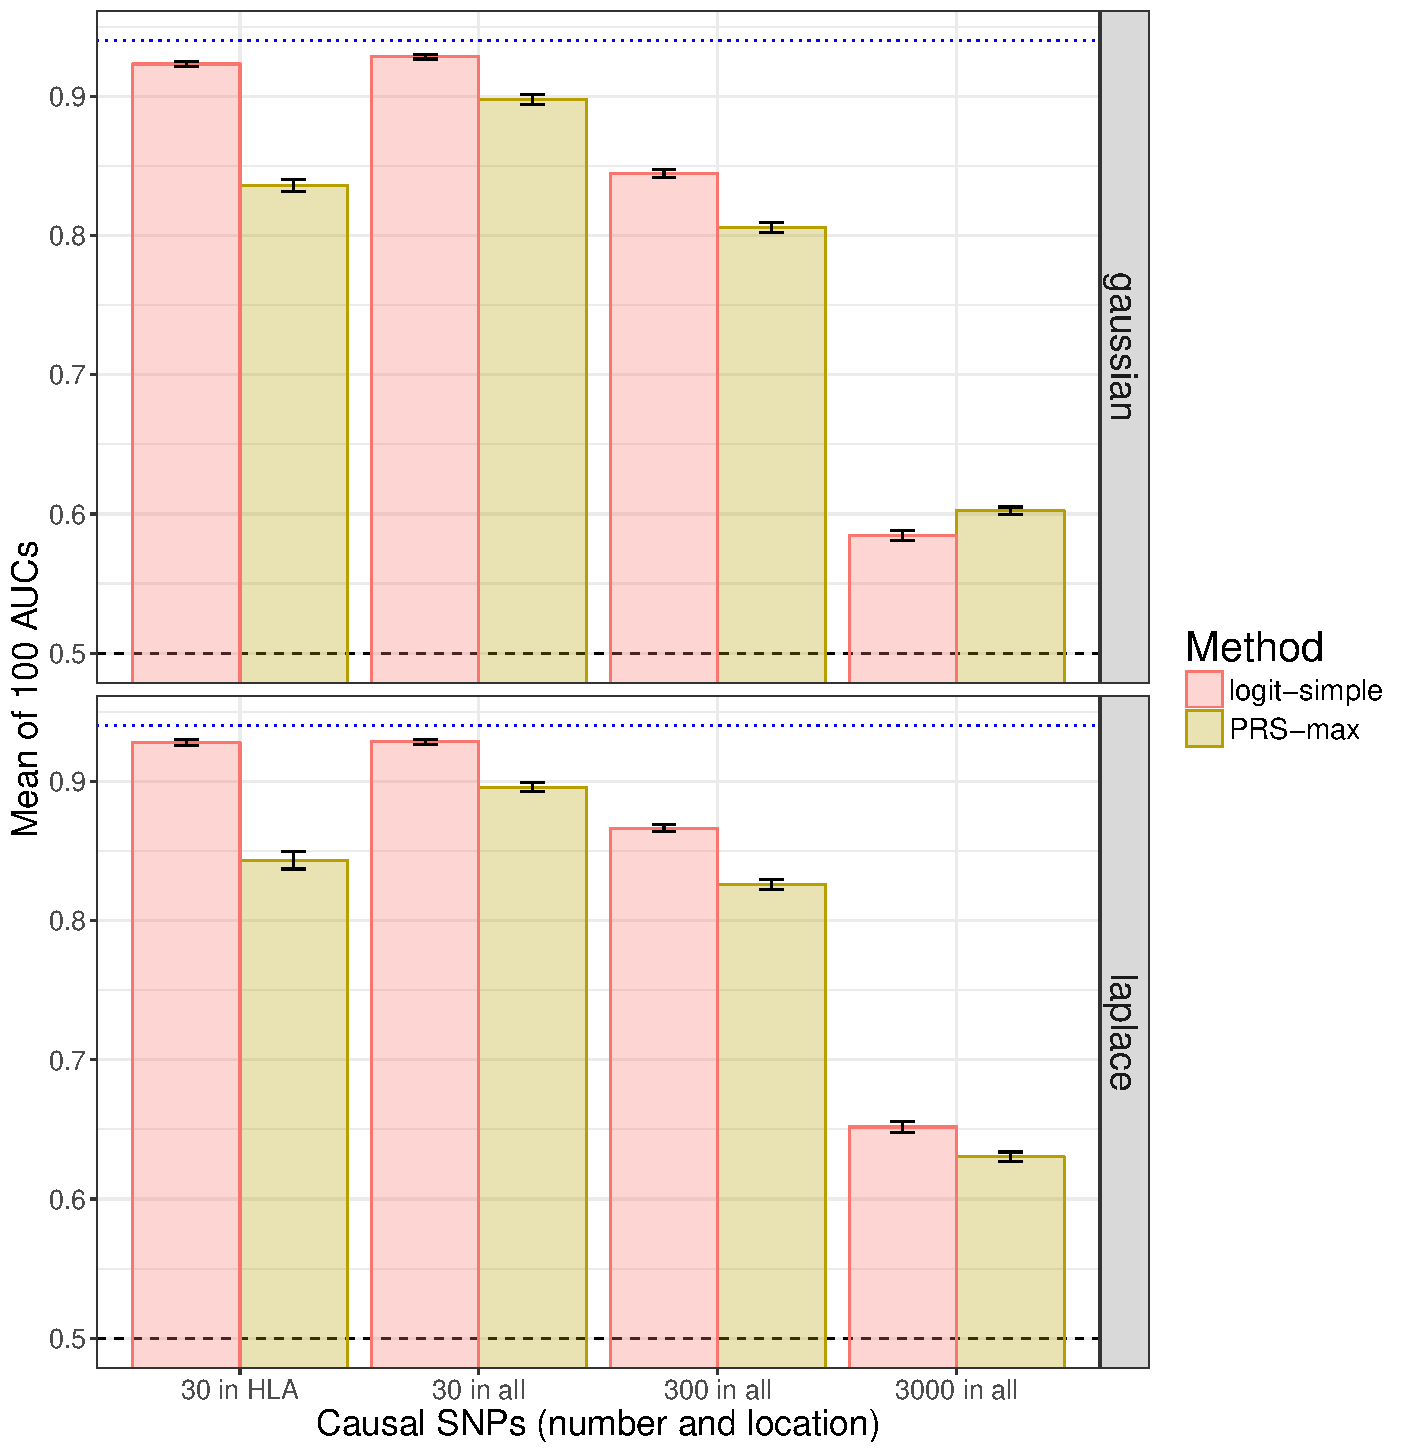
\includegraphics[width=\textwidth]{main-AUC-logit}}
\caption{Scenario \textnumero1. Mean of AUC over 100 simulations for our penalized logistic regression (``logit-simple'') and the maximum AUC reported with the C+T method (``PRS-max''). Upper (lower) panel is presenting results for effets following a Gaussian (Laplace) distribution. Error bars are representing $\pm 2 \text{SD}$ of $10^5$ non-parametric bootstrap of the mean of AUC. The blue dotted line represents the maximum achievable AUC. [MODEL AND H2]}
\label{fig:main-AUC-logit}
\end{figure}

\newpage
\begin{figure}[h]
\centerline{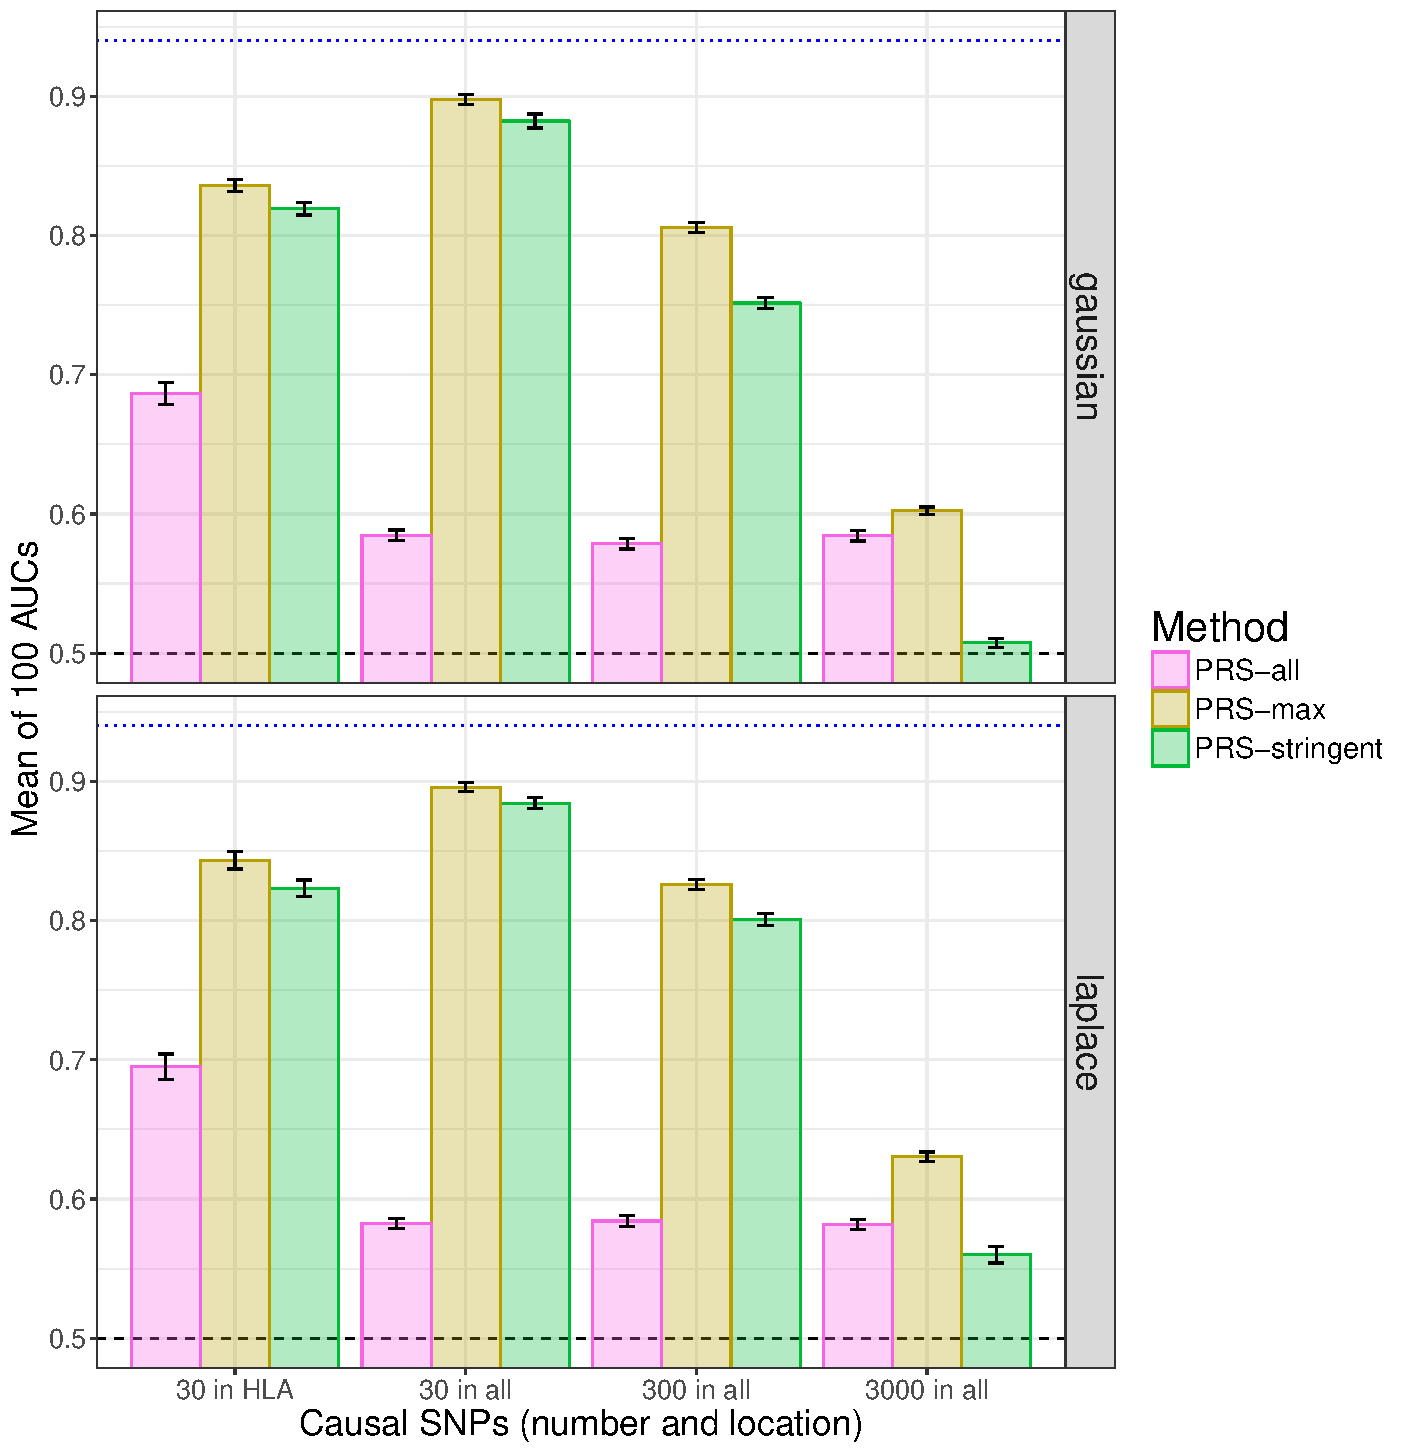
\includegraphics[width=\textwidth]{main-AUC-PRS}}
\caption{Scenario \textnumero1. Mean of AUC over 100 simulations for ..the three reported PRSs... Upper (lower) panel is presenting results for effets following a Gaussian (Laplace) distribution. Error bars are representing $\pm 2 \text{SD}$ of $10^5$ non-parametric bootstrap of the mean of AUC. The blue dotted line represents the maximum achievable AUC. [MODEL AND H2]}
\label{fig:main-AUC-PRS}
\end{figure}

\newpage
\begin{figure}[h]
\centerline{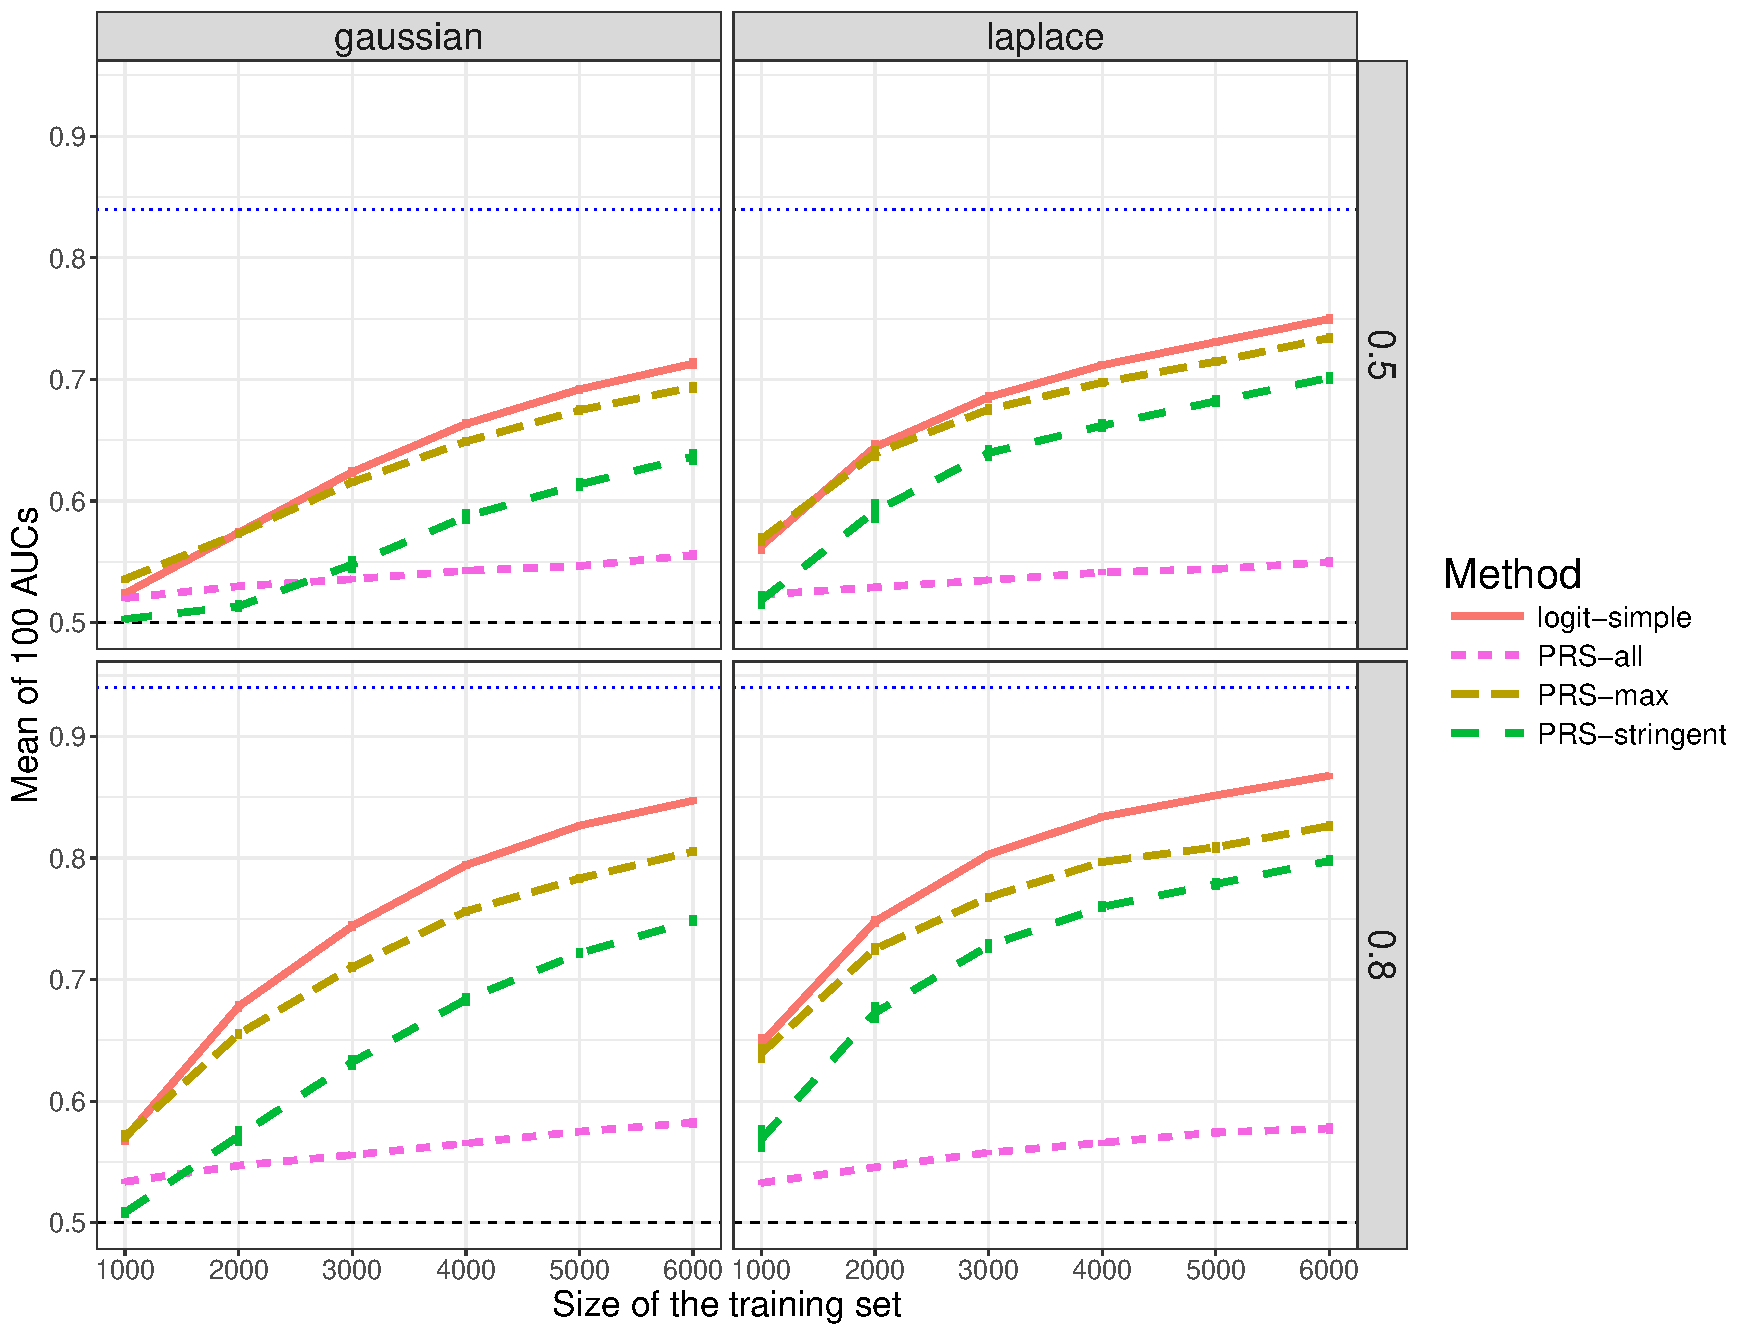
\includegraphics[width=\textwidth]{main-AUC-ntrain}}
\caption{Scenario \textnumero3. Mean of AUC over 100 simulations for ..the three reported PRSs... and the simple logistic regression as a function of the training size. This results are for an additive model with 300 causal SNPs sampled anywhere on the genome. Upper (lower) panels are presenting results for an heritability of 0.5 (0.8) and left (right) panels are presenting results for effets following a Gaussian (Laplace) distribution. Error bars are representing $\pm 2 \text{SD}$ of $10^5$ non-parametric bootstrap of the mean of AUC. The blue dotted line represents the maximum achievable AUC. [MODEL AND H2]}
\label{fig:main-AUC-ntrain}
\end{figure}

\newpage
\begin{figure}[h]
\centerline{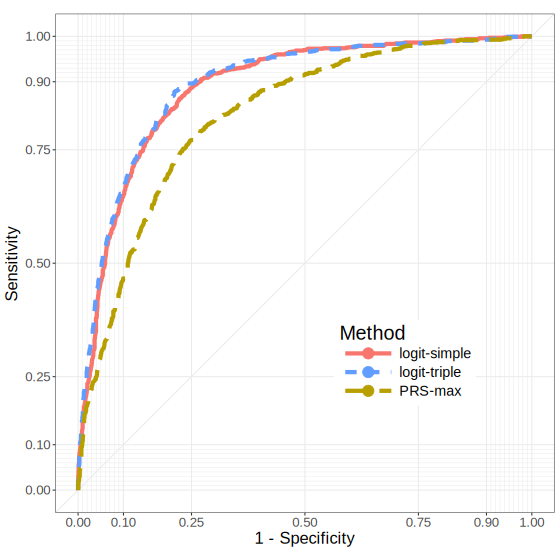
\includegraphics[width=\textwidth]{celiac-roc}}
\caption{ROC Curves for the ``C+T'', ``logit-simple'' and ``logit-triple'' methods for one run on the Celiac disease, training on 12,000 individuals and projecting on the remaining 3155 individuals. Plotted using R package plotROC \cite[]{sachs2017plotroc}.\label{fig:celiac-roc}}
\end{figure}

%%%%%%%%%%%%%%%%%%%%%%%%%%%%%%%%%%%%%%%%%%%%%%%%%%%%%%%%%%%%%%%%%%%%%%%%%%%%%%%%

\clearpage
\section*{Acknowledgements}

Authors acknowledge Grenoble Alpes Data Institute, supported by the French National Research Agency under the ``Investissements d'avenir'' program (ANR-15-IDEX-02) and the LabEx PERSYVAL-Lab (ANR-11-LABX-0025-01). We are also grateful to F\'elix Balazard for useful discussions about T-Trees, and to Yaohui Zeng for useful discussions about R package biglasso.

\vspace*{-12pt}

\bibliographystyle{natbib}
\bibliography{refs}

%%%%%%%%%%%%%%%%%%%%%%%%%%%%%%%%%%%%%%%%%%%%%%%%%%%%%%%%%%%%%%%%%%%%%%%%%%%%%%%%
%%%%%%%%%%%%%%%%%%%%%%%%%%%%%%%%%%%%%%%%%%%%%%%%%%%%%%%%%%%%%%%%%%%%%%%%%%%%%%%%
%%%%%%%%%%%%%%%%%%%%%%%%%%%%%%%%%%%%%%%%%%%%%%%%%%%%%%%%%%%%%%%%%%%%%%%%%%%%%%%%

\newpage
\section*{Supplementary Materials}

\renewcommand{\thefigure}{S\arabic{figure}}
\setcounter{figure}{0}
\renewcommand{\thetable}{S\arabic{table}}
\setcounter{table}{0}

%%%%%%%%%%%%%%%%%%%%%%%%%%%%%%%%%%%%%%%%%%%%%%%%%%%%%%%%%%%%%%%%%%%%%%%%%%%%%%%%

\subsection*{Maximum AUCs} \label{sec:auc-max}

We used three different ways to estimate the maximum achievable AUC for our simulations.
First, we used the estimation from equation (3) of \cite{wray2010genetic}. For a prevalence fixed at 30\% and an heritability of 50\% (respectively 80\%), the approximated theoretical values of AUC are 84.1\% (respectively 93.0\%). Note that this approximation is reported to be less accurate for high heritabilities.
Secondly, if we assume that the genetic part of the liabilities $y \sim N(0, h^2)$, we can estimate the theoretical value of the AUC that can be achieved given the heritability $h^2$ through Monte Carlo simulations. We report AUCs of 84.1\% and 94.1\% for respectively an heritability of 50\% and 80\%. [HOW TO ADD ERROR? I HAVE SUMMARY()]
Thirdly, we reproduce the exact same procedure of simulations and, for each combination of parameters (Table \ref{tab:simus}), we estimate the AUC of the ``oracle'', i.e.\ the true simulated genetic part of the liabilities though 100 replicates. For every combination of parameters, AUC of oracles are comprised between 83.2\% and 84.2\% for an heritability of 50\% and between 93.2\% and 94.1\% for an heritability of 80\%.
Given all these estimates of the maximal achievable AUC and for the sake of simplicity, we report maximum AUCs of 84\% (94\%) for heritabilities of 50\% (80\%) whatever are the parameters of the simulation.


%%%%%%%%%%%%%%%%%%%%%%%%%%%%%%%%%%%%%%%%%%%%%%%%%%%%%%%%%%%%%%%%%%%%%%%%%%%%%%%%

\newpage

\begin{table}[ht]
\centering
\begin{tabular}{|l|cccc|r|}
\hline
Population & UK & Finland & Netherlands & Italy & Total\\
\hline
Cases & 2569 & 637 & 795 & 495 & 4496\\
Controls & 7492 & 1799 & 828 & 540 & 10659\\
\hline
Total & 10061 & 2436 & 1623 & 1035 & 15155\\
\hline
\end{tabular}
\caption{Number of individuals by population and disease status for the celiac disease cohort (after quality control, genotyped on 281,122 ..mutual.. SNPs).\label{tab:celiac-data}}
\end{table}

%%%%%%%%%%%%%%%%%%%%%%%%%%%%%%%%%%%%%%%%%%%%%%%%%%%%%%%%%%%%%%%%%%%%%%%%%%%%%%%%

% latex table generated in R 3.4.1 by xtable 1.8-2 package
% Thu Oct 26 16:46:26 2017
\begin{table}[ht]
\centering
\begin{tabular}{ccccccccccccccc}
  \hline
1.00e+00 & 7.22e-01 & 5.87e-01 & 4.20e-01 & 2.43e-01 & 1.00e-01 & 2.35e-02 & 2.21e-03 & 4.69e-05 & 8.81e-08 & 3.18e-12 & 1.83e-19 & 2.89e-31 & 1.70e-50 & 7.71e-82 \\ 
  5.00e-08 & 7.05e-01 & 5.65e-01 & 3.95e-01 & 2.20e-01 & 8.47e-02 & 1.79e-02 & 1.42e-03 & 2.28e-05 & 2.73e-08 & 4.69e-13 & 8.08e-21 & 1.80e-33 & 4.30e-54 & 1.06e-87 \\ 
  7.94e-01 & 6.87e-01 & 5.42e-01 & 3.69e-01 & 1.97e-01 & 7.08e-02 & 1.34e-02 & 8.83e-04 & 1.05e-05 & 7.74e-09 & 6.03e-14 & 2.86e-22 & 7.73e-36 & 5.97e-58 & 5.49e-94 \\ 
  7.81e-01 & 6.69e-01 & 5.19e-01 & 3.43e-01 & 1.75e-01 & 5.85e-02 & 9.79e-03 & 5.31e-04 & 4.61e-06 & 2.01e-09 & 6.69e-15 & 7.92e-24 & 2.24e-38 & 4.37e-62 & 1.00e-100 \\ 
  7.67e-01 & 6.50e-01 & 4.95e-01 & 3.18e-01 & 1.54e-01 & 4.76e-02 & 7.01e-03 & 3.08e-04 & 1.90e-06 & 4.72e-10 & 6.32e-16 & 1.70e-25 & 4.26e-41 & 1.61e-66 &  \\ 
  7.53e-01 & 6.30e-01 & 4.70e-01 & 2.93e-01 & 1.35e-01 & 3.82e-02 & 4.90e-03 & 1.72e-04 & 7.31e-07 & 1.00e-10 & 5.04e-17 & 2.75e-27 & 5.16e-44 & 2.83e-71 &  \\ 
  7.38e-01 & 6.09e-01 & 4.46e-01 & 2.68e-01 & 1.17e-01 & 3.02e-02 & 3.33e-03 & 9.18e-05 & 2.63e-07 & 1.89e-11 & 3.35e-18 & 3.31e-29 & 3.84e-47 & 2.26e-76 &  \\ 
   \hline
\end{tabular}
\caption{The 102 thresholds used in the C+T method for this study.\label{tab:thr}}
\end{table}

%%%%%%%%%%%%%%%%%%%%%%%%%%%%%%%%%%%%%%%%%%%%%%%%%%%%%%%%%%%%%%%%%%%%%%%%%%%%%%%%

\newpage
\begin{figure}[h]
\centerline{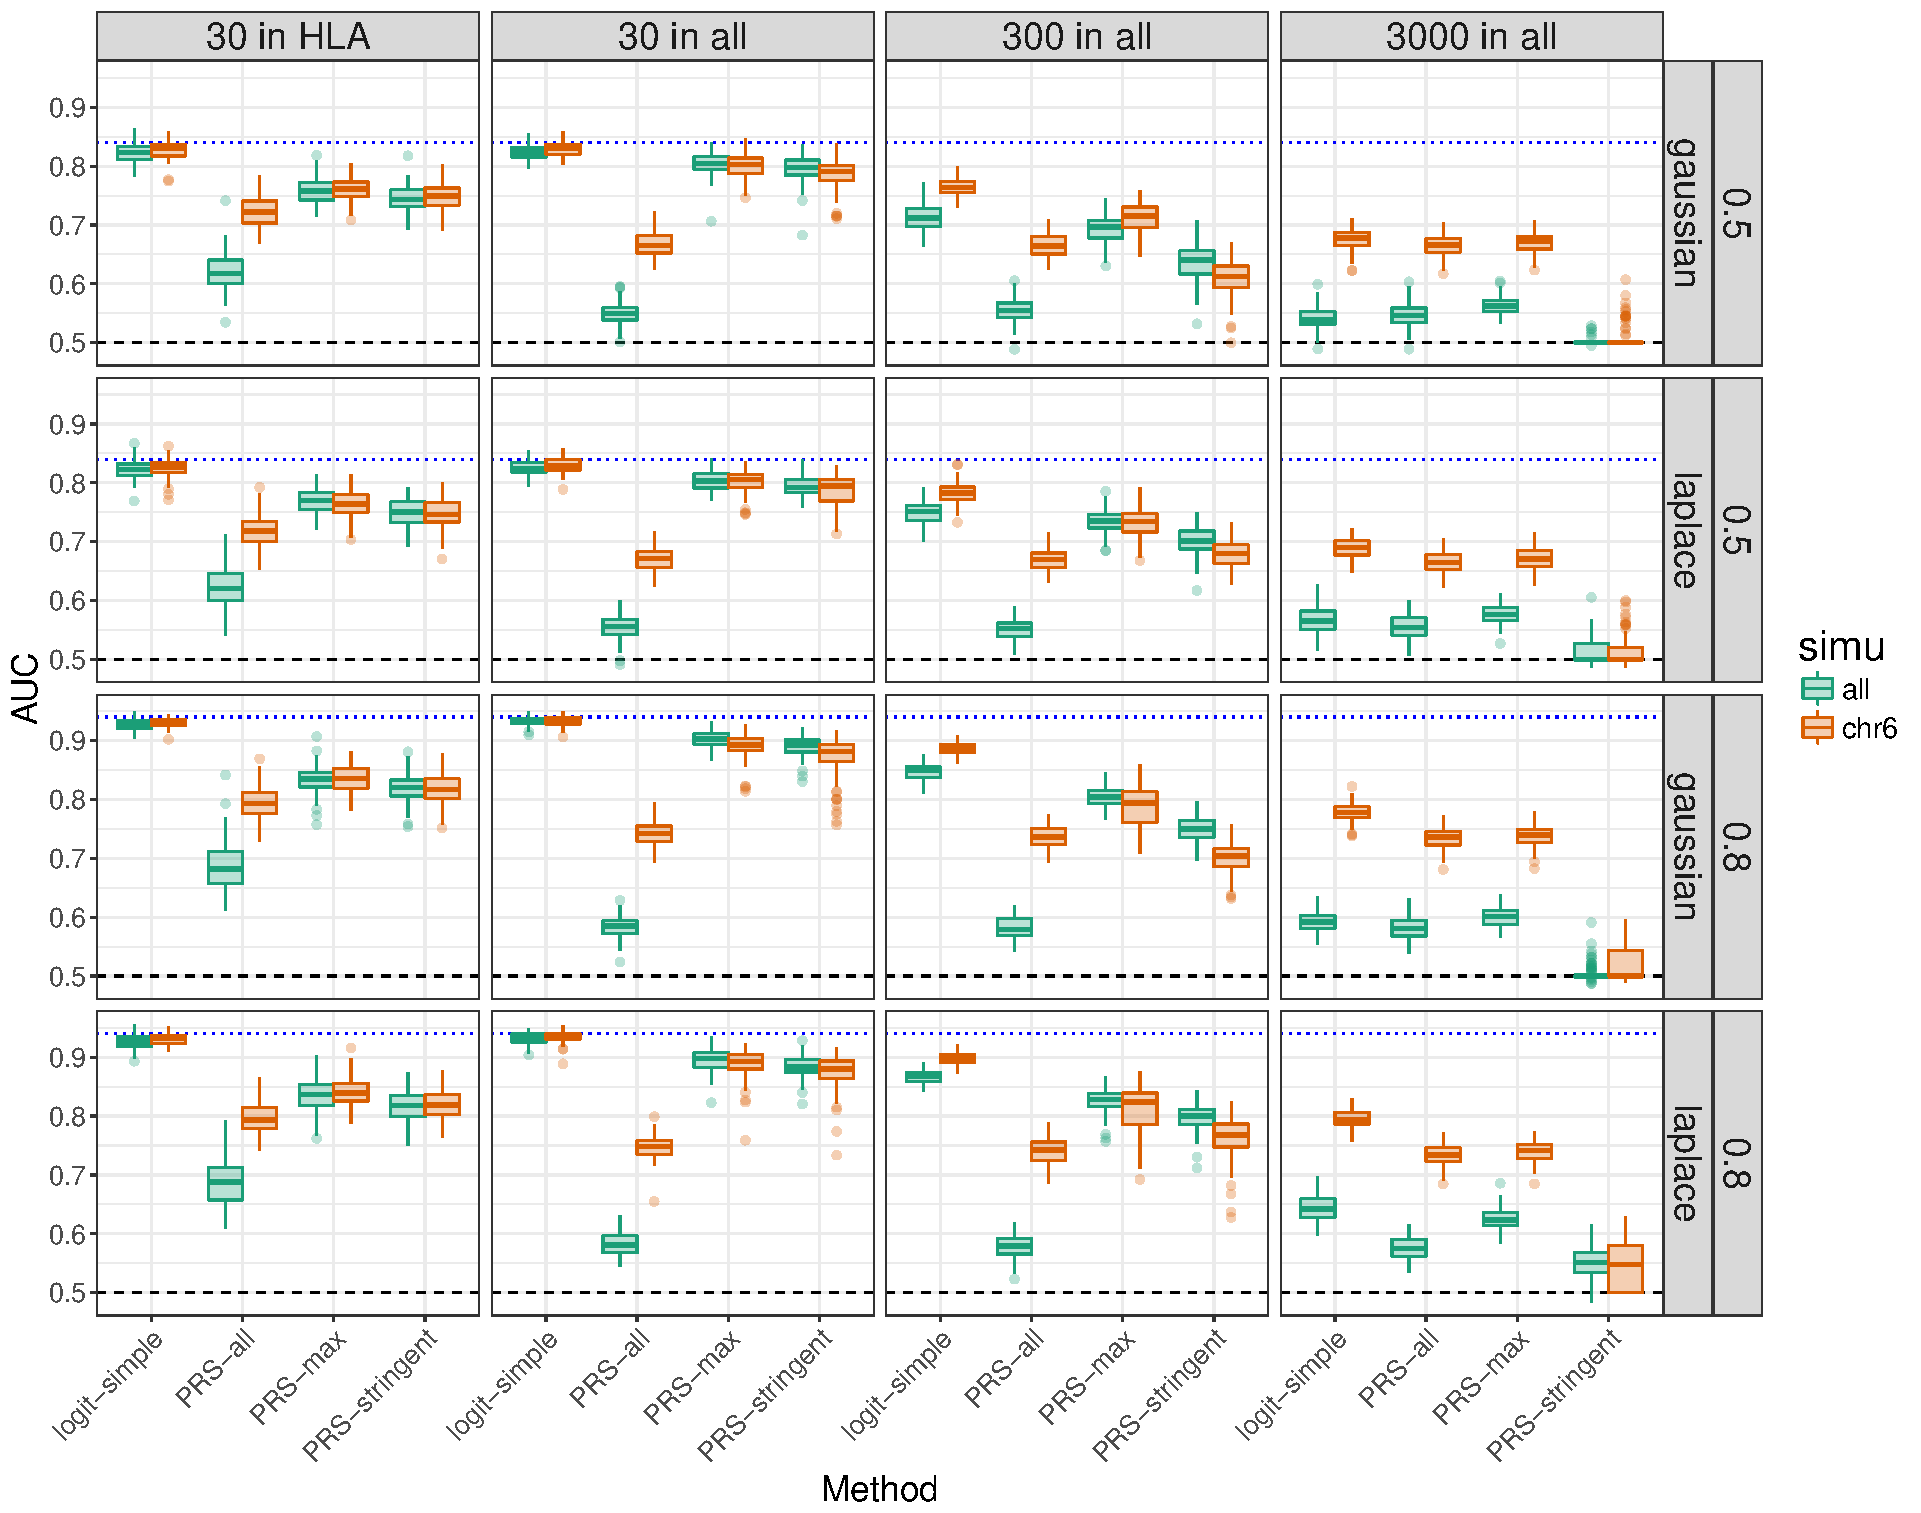
\includegraphics[width=\textwidth]{supp-AUC-chr6}}
\caption{Scenario \textnumero2. Boxplots of AUC over 100 simulations for ..the three reported PRSs... and the simple logistic regression.
Vertical panels represents different number of causal SNPs and their location (``all'': anywhere on the genome; ``HLA'': only in the HLA region). Horizontal panels are presenting results for effets following a Gaussian or Laplace distribution and an heritability of 0.5 or 0.8. The blue dotted line represents the maximum achievable AUC. [MODEL AND H2]}
\label{fig:supp-AUC-chr6}
\end{figure}

%%%%%%%%%%%%%%%%%%%%%%%%%%%%%%%%%%%%%%%%%%%%%%%%%%%%%%%%%%%%%%%%%%%%%%%%%%%%%%%%

\newpage
\begin{figure}[h]
\centerline{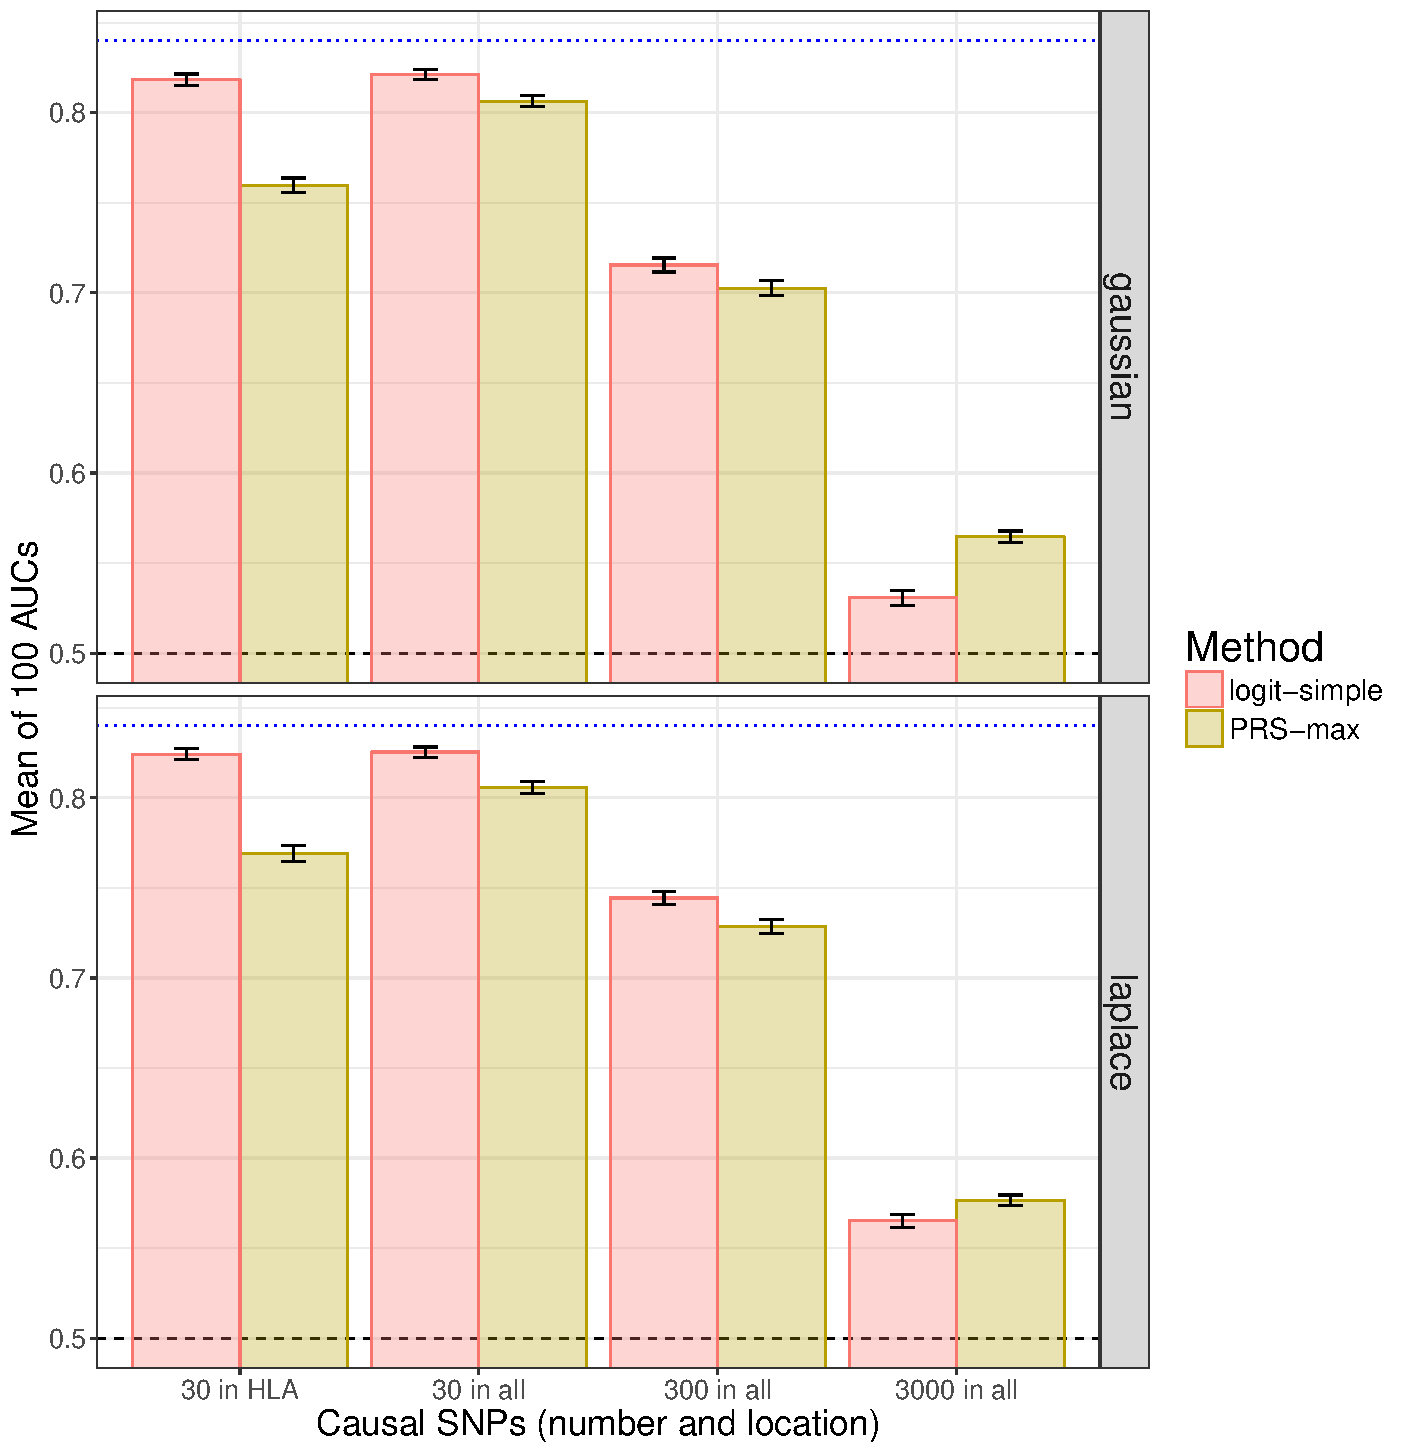
\includegraphics[width=\textwidth]{supp-AUC-logit}}
\caption{[COPY FOR H2=0.5]}
\label{fig:supp-AUC-logit}
\end{figure}

\newpage
\begin{figure}[h]
\centerline{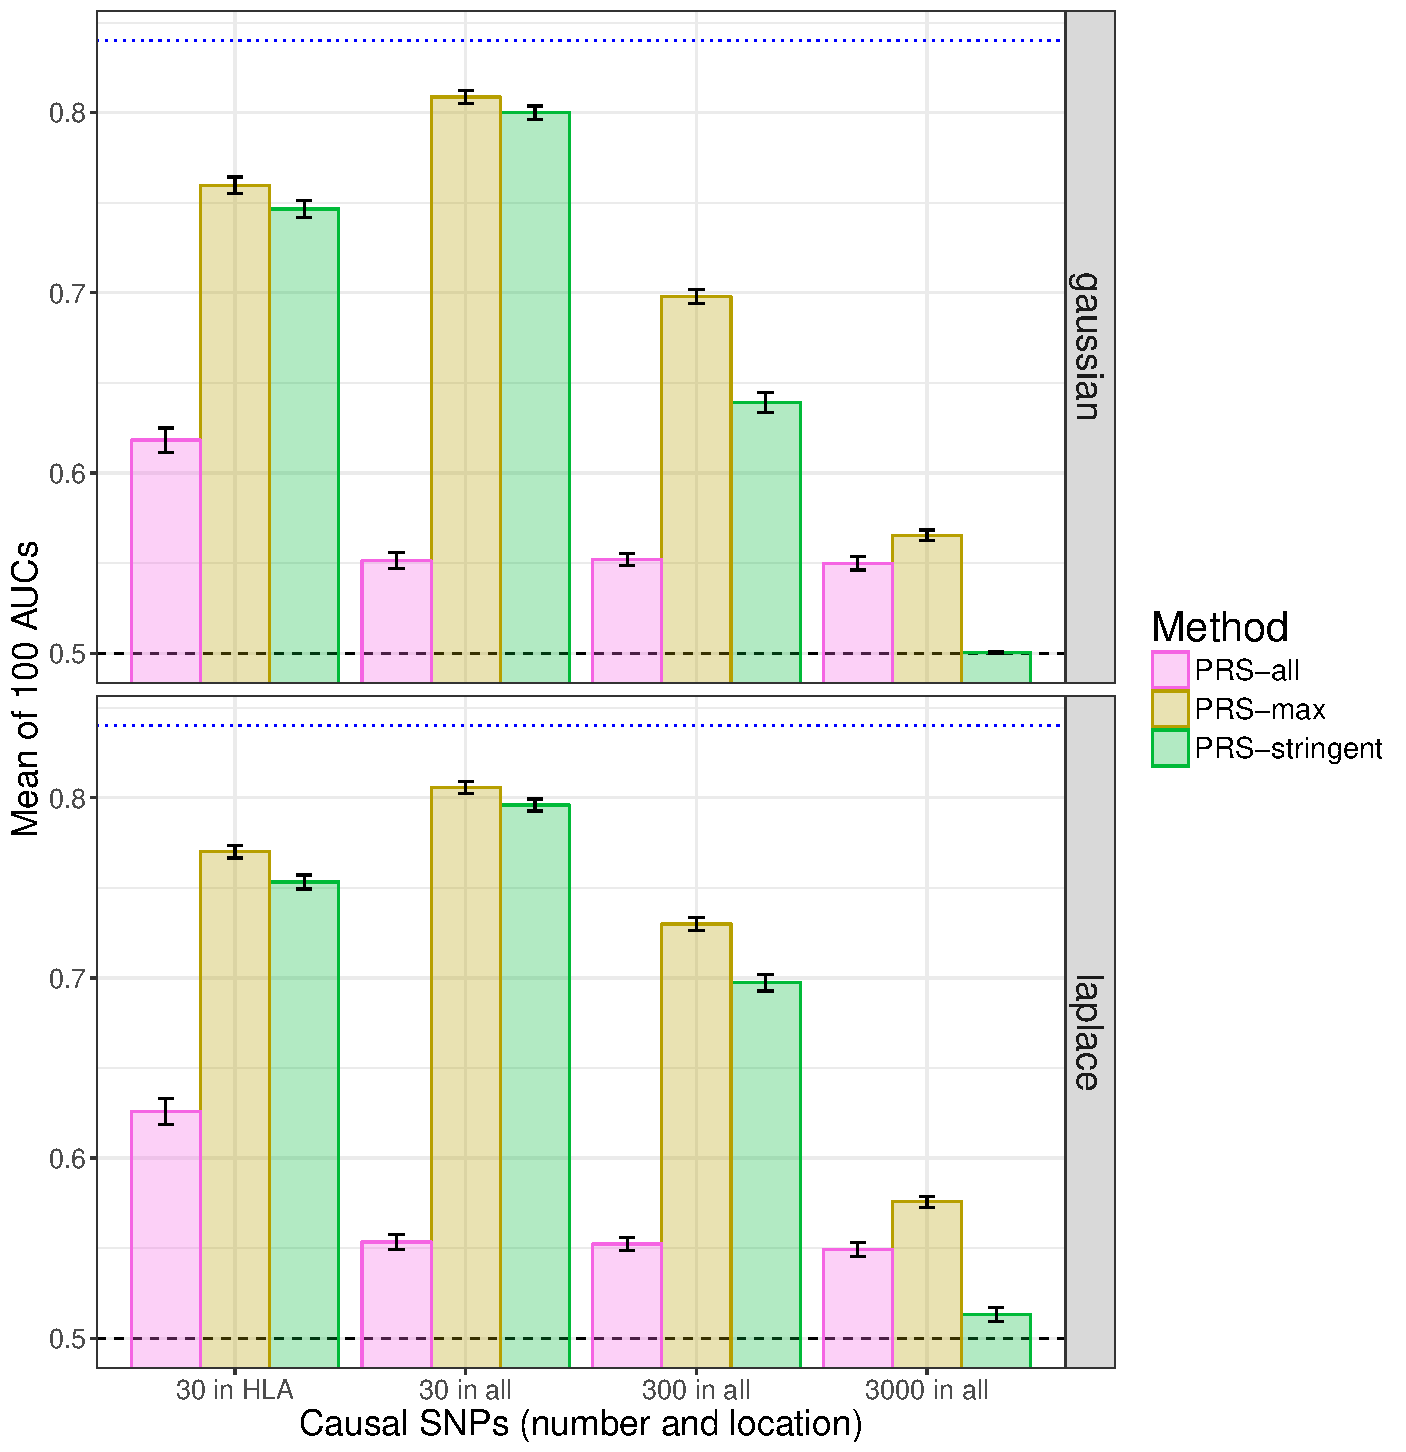
\includegraphics[width=\textwidth]{supp-AUC-PRS}}
\caption{[COPY FOR H2=0.5]}
\label{fig:supp-AUC-PRS}
\end{figure}

%%%%%%%%%%%%%%%%%%%%%%%%%%%%%%%%%%%%%%%%%%%%%%%%%%%%%%%%%%%%%%%%%%%%%%%%%%%%%%%%

\newpage
\begin{figure}[h]
\centerline{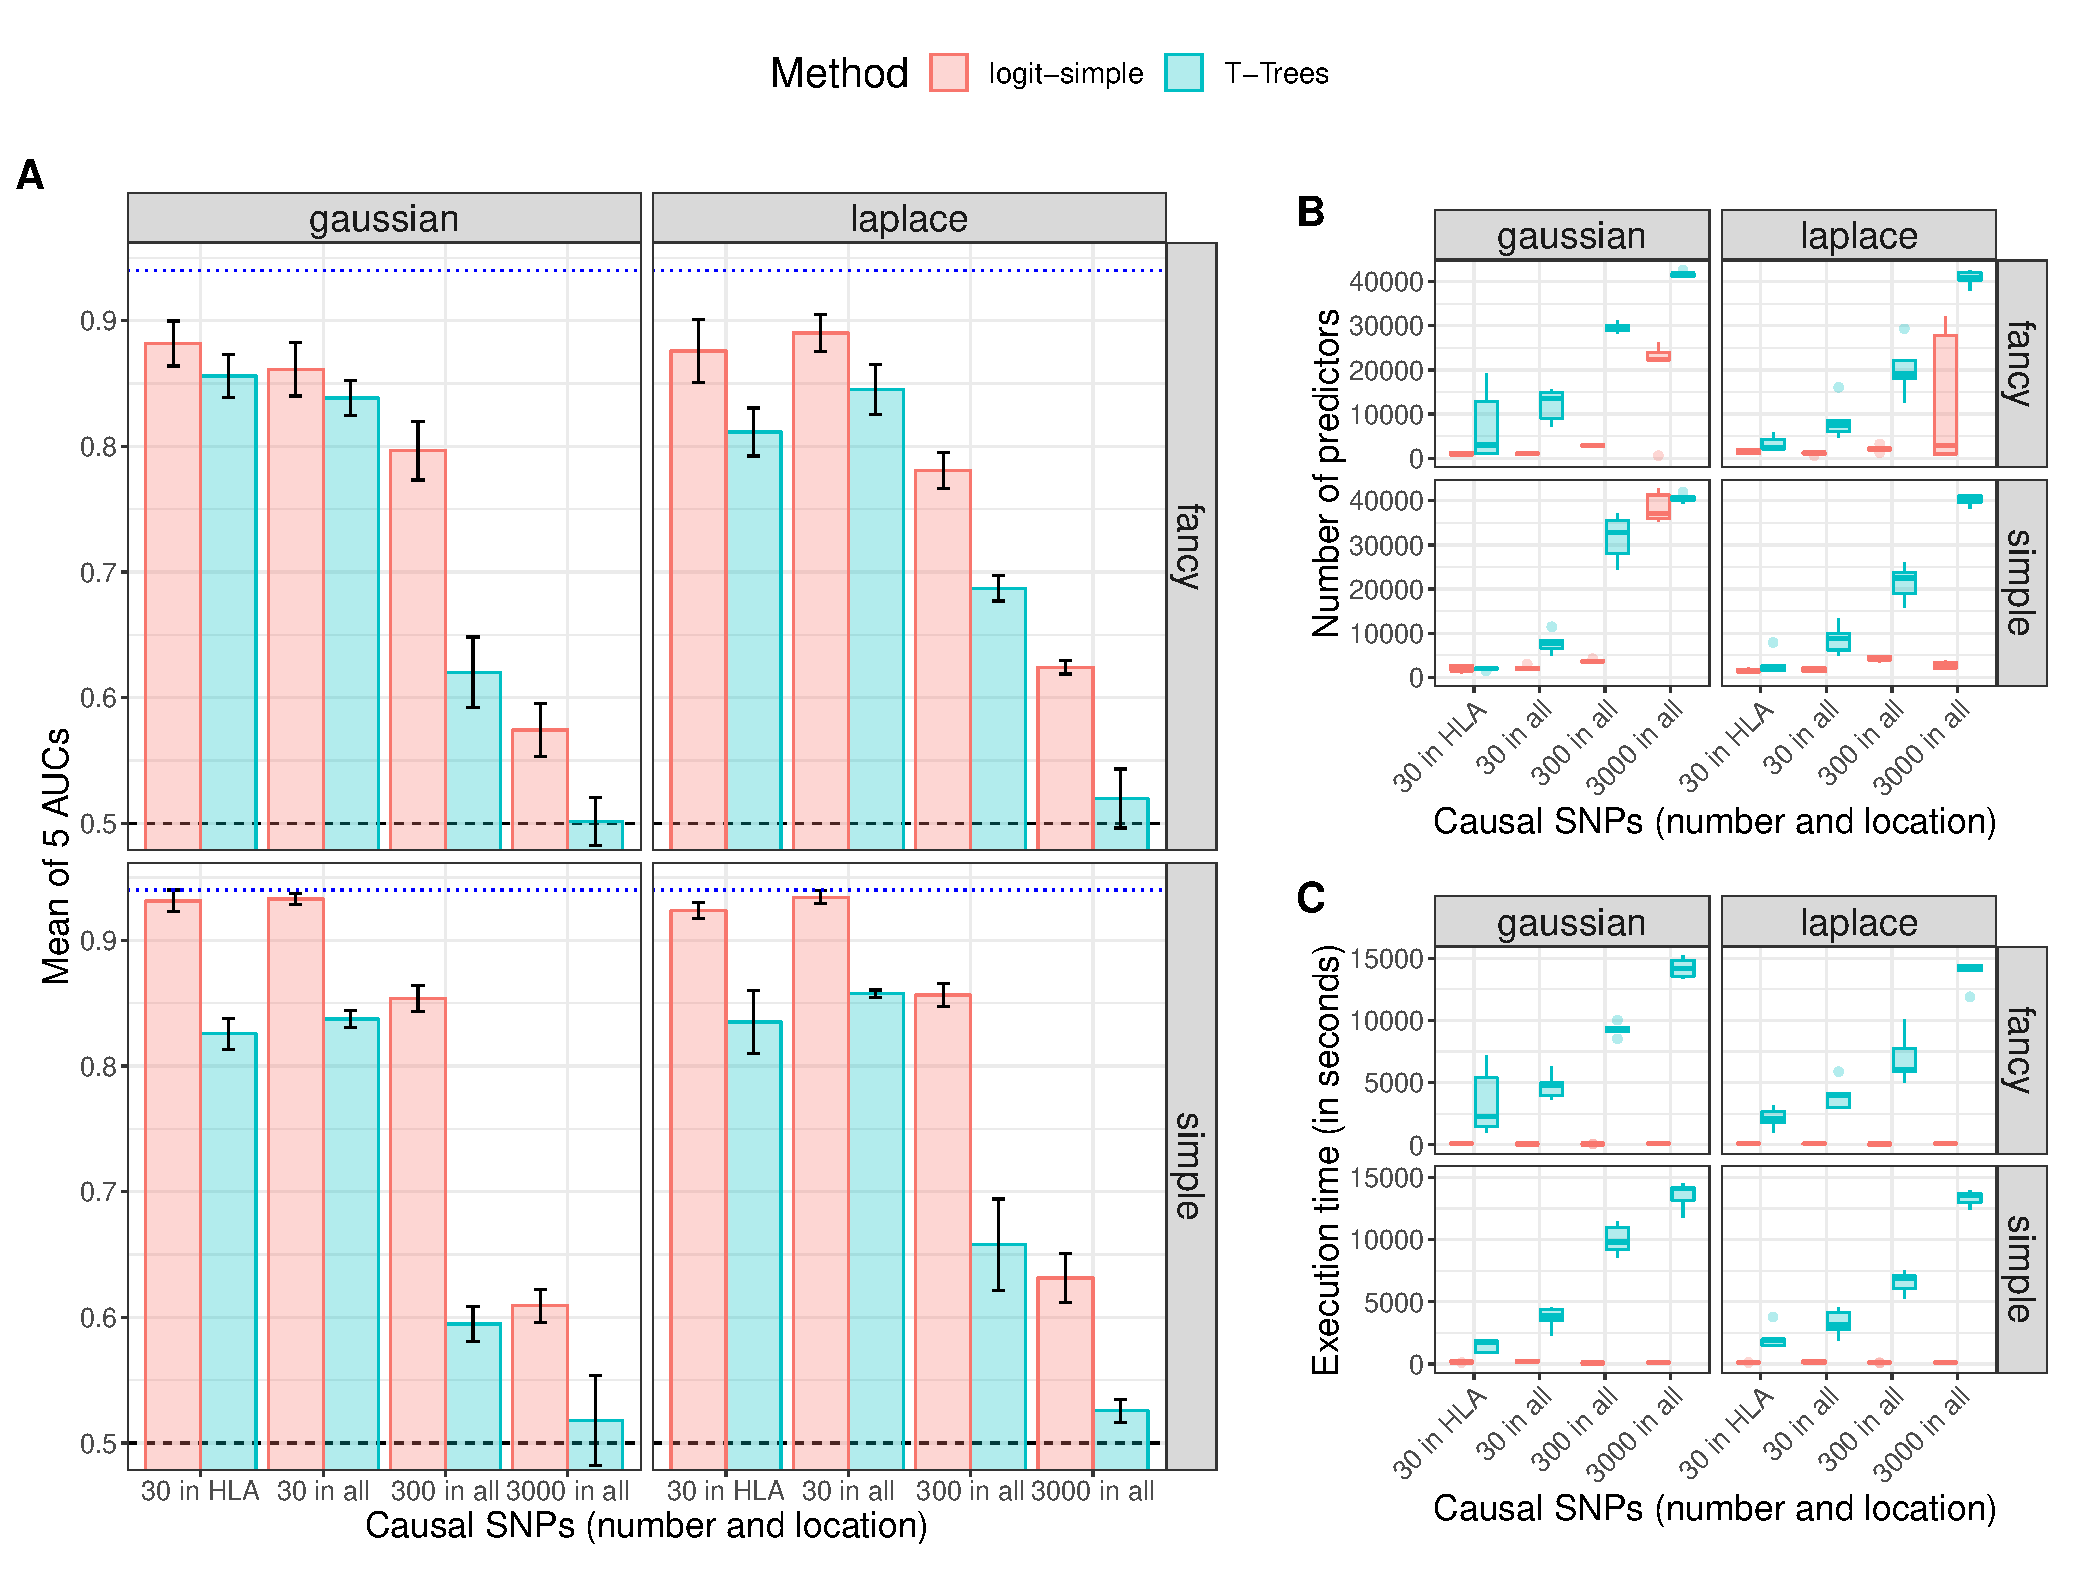
\includegraphics[width=\textwidth]{supp-ttrees}}
\caption{[T-TREES 3 PLOTS - H2=0.8]}
\label{fig:supp-ttrees}
\end{figure}

\newpage
\begin{figure}[h]
\centerline{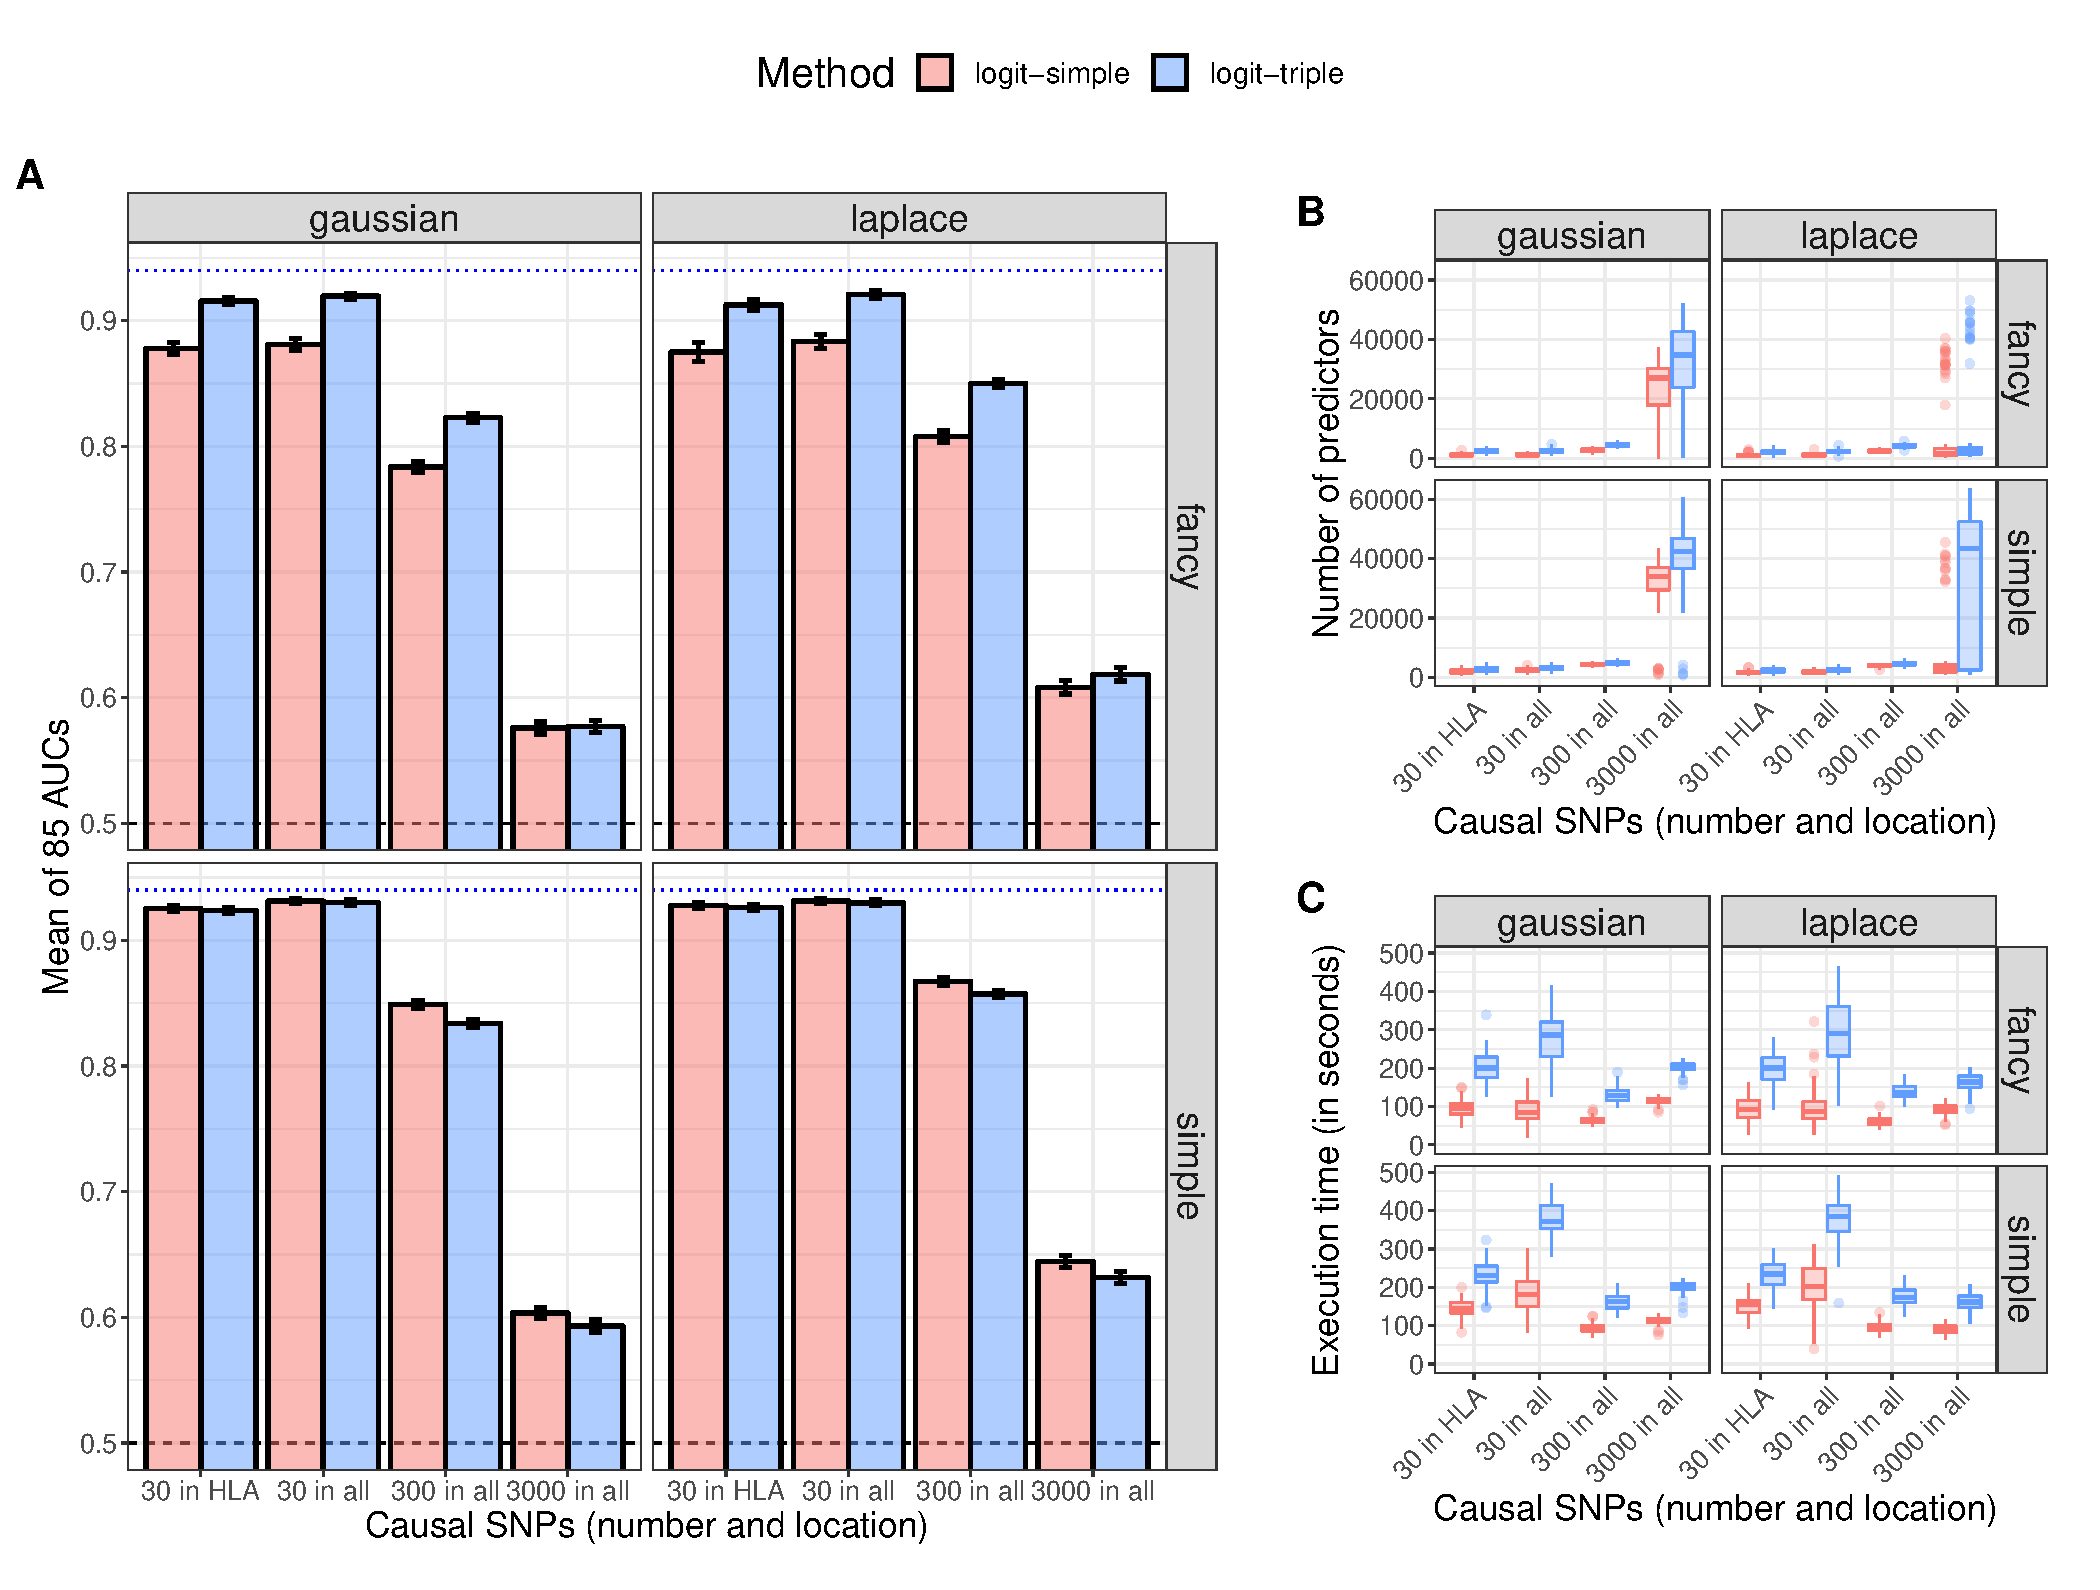
\includegraphics[width=\textwidth]{supp-triple}}
\caption{[TRIPLE 3 PLOTS - H2=0.8]}
\label{fig:supp-triple}
\end{figure}

\newpage
\begin{figure}[h]
\centerline{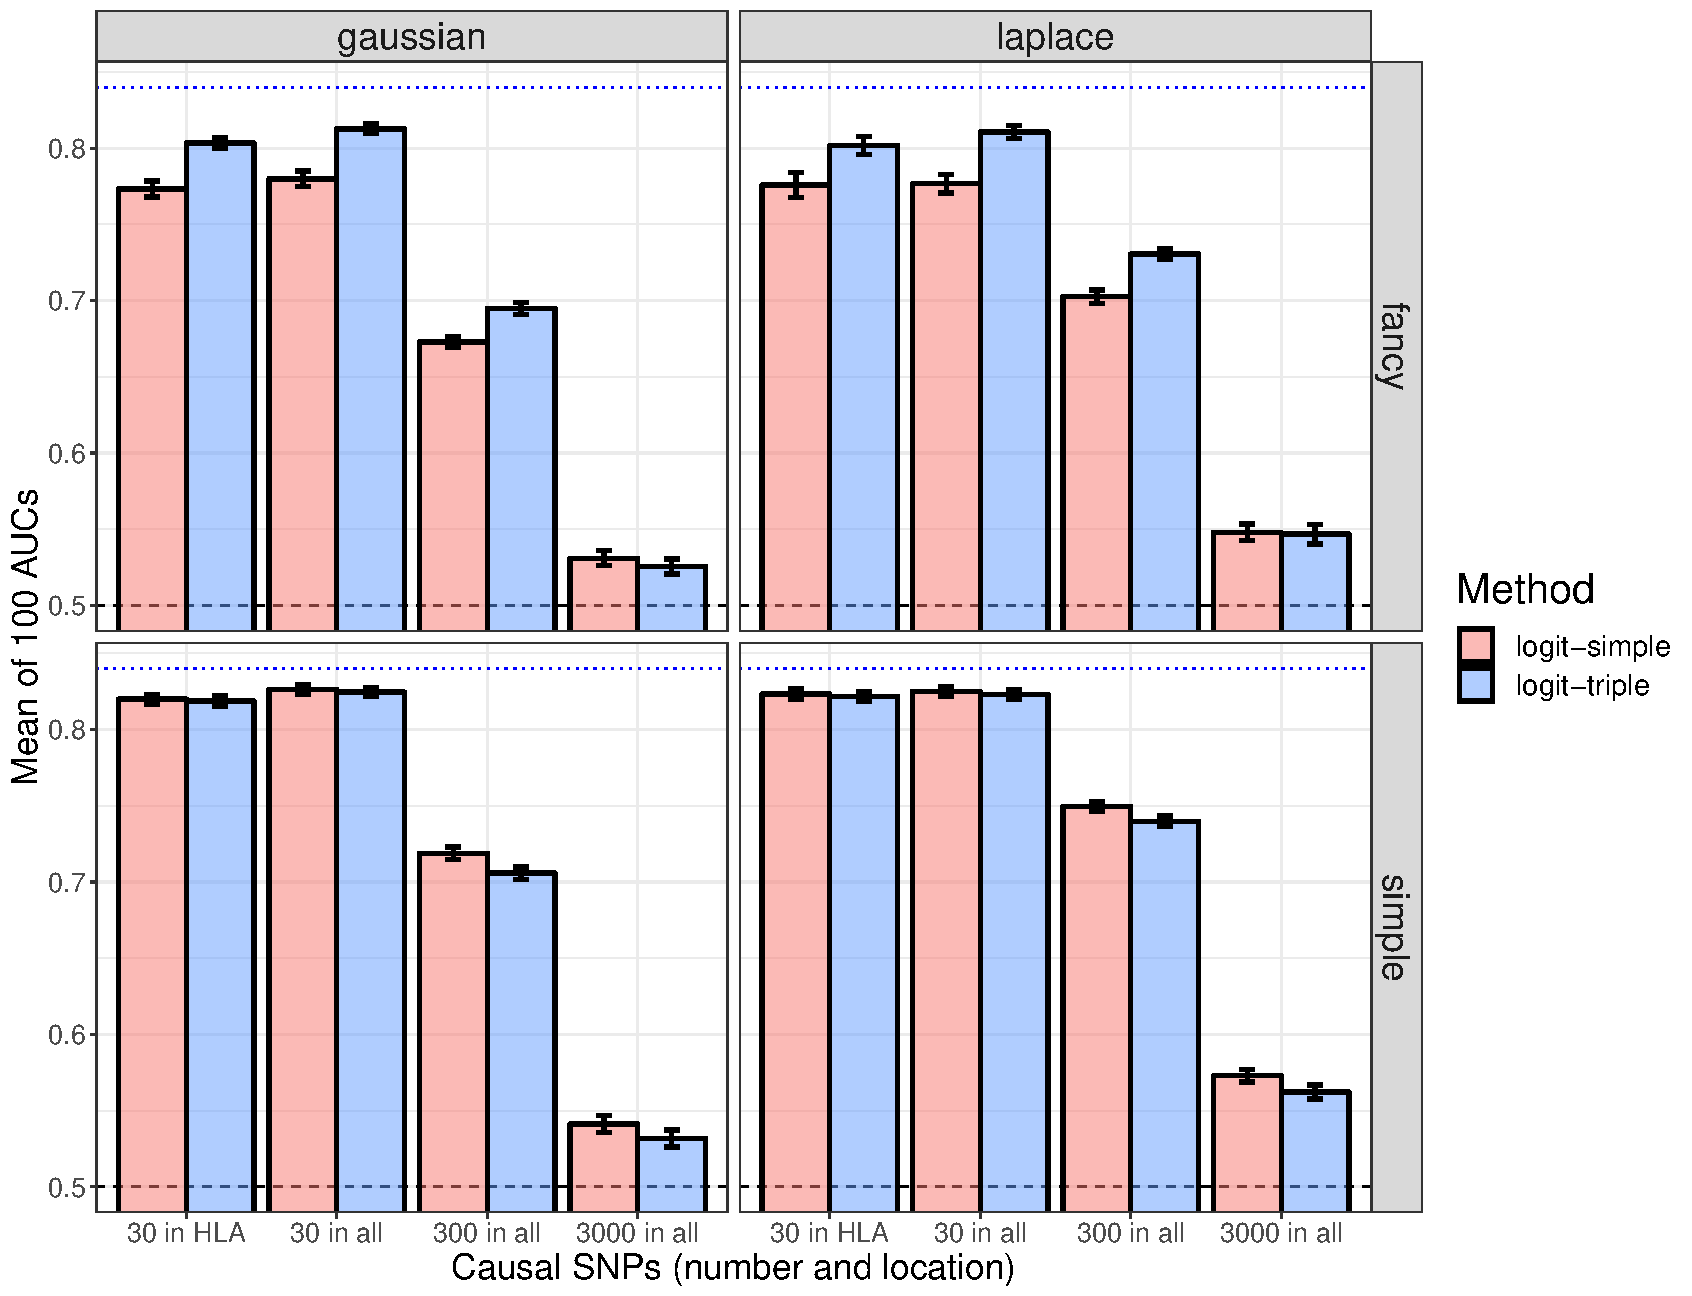
\includegraphics[width=\textwidth]{supp-AUC-triple}}
\caption{[TRIPLE ONLY AUC - H2=0.5]}
\label{fig:supp-AUC-triple}
\end{figure}

\newpage
\begin{figure}[h]
\centerline{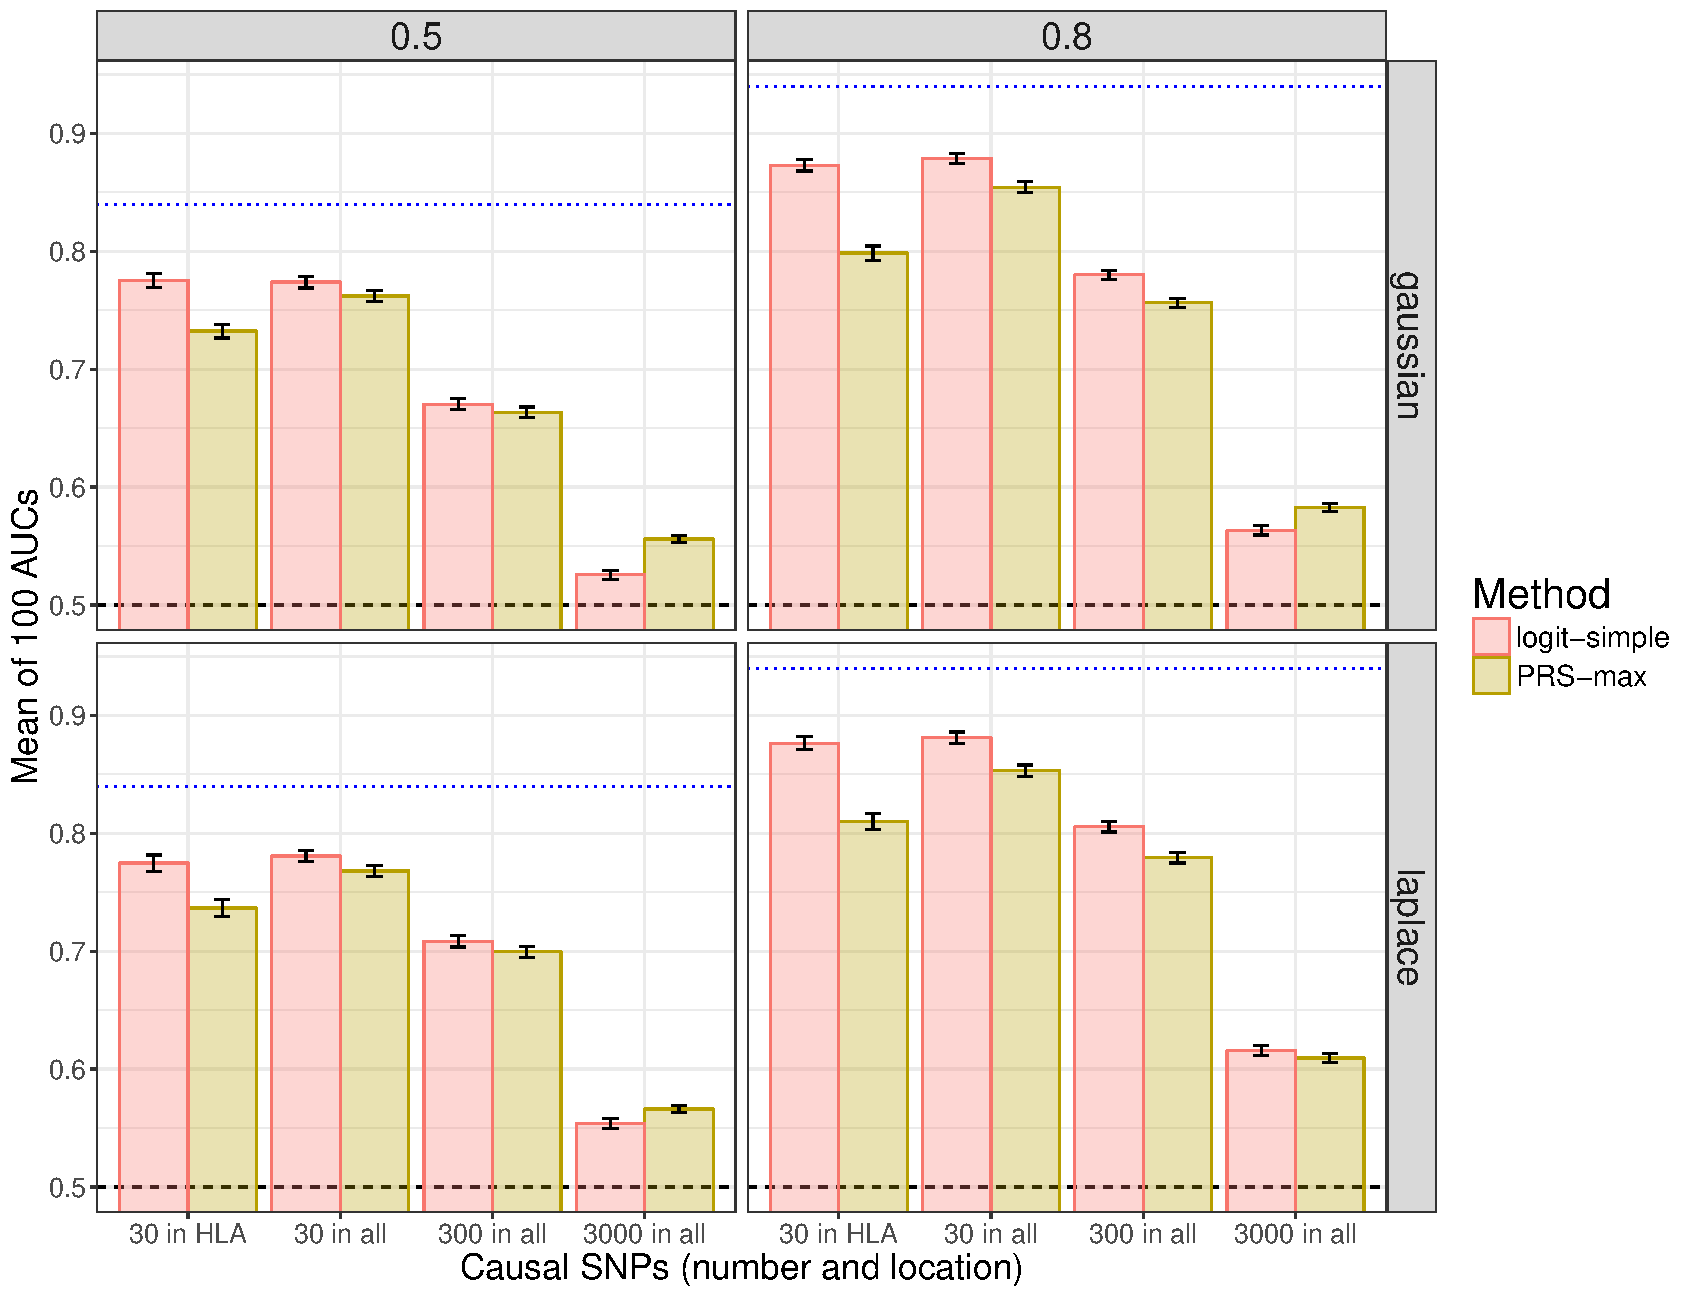
\includegraphics[width=\textwidth]{supp-AUC-logit-fancy}}
\caption{[COPY FOR H2=0.5 \& MODEL FANCY]}
\label{fig:supp-AUC-logit-fancy}
\end{figure}

\newpage
\begin{figure}[h]
\centerline{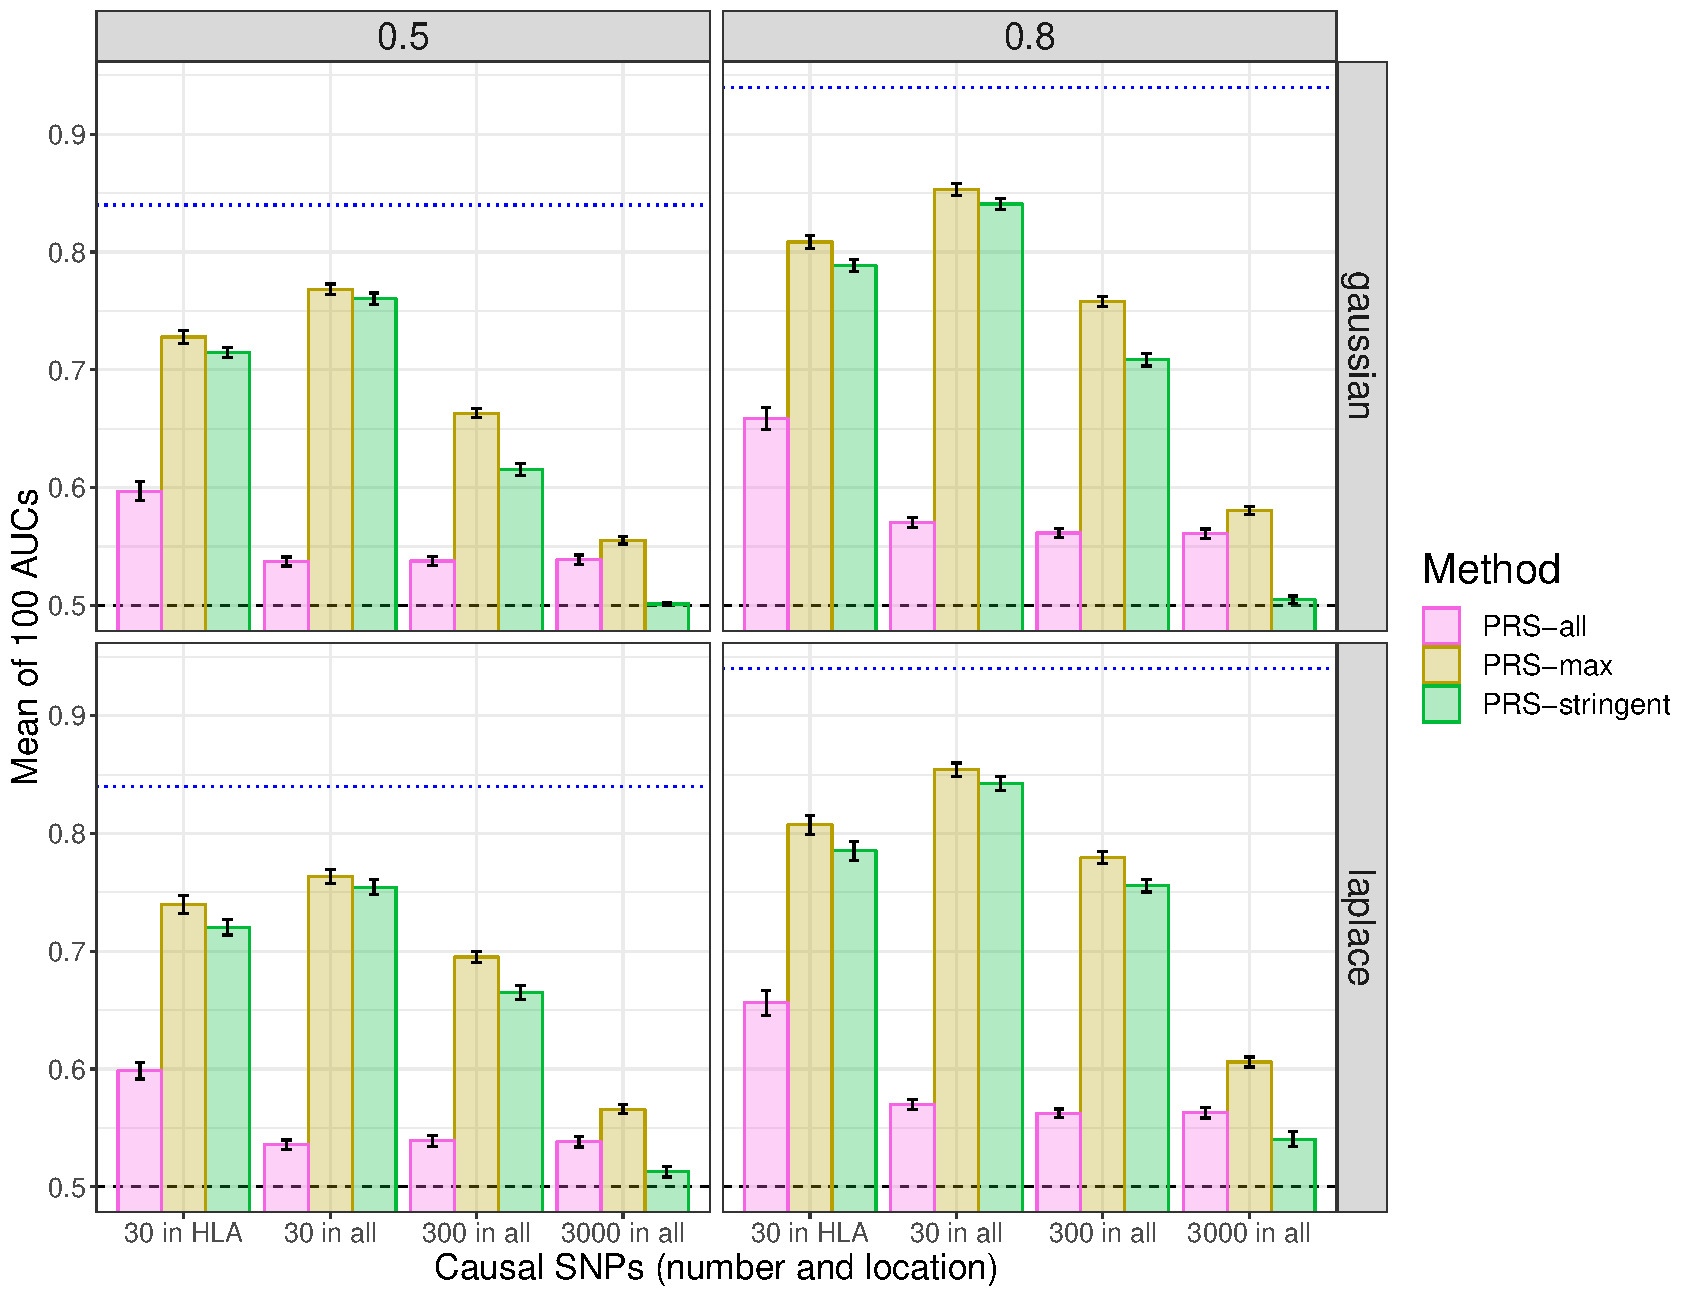
\includegraphics[width=\textwidth]{supp-AUC-PRS-fancy}}
\caption{[COPY FOR H2=0.5 \& MODEL FANCY]}
\label{fig:supp-AUC-PRS-fancy}
\end{figure}

%%%%%%%%%%%%%%%%%%%%%%%%%%%%%%%%%%%%%%%%%%%%%%%%%%%%%%%%%%%%%%%%%%%%%%%%%%%%%%%%

\newpage
\begin{figure}[h]
\centerline{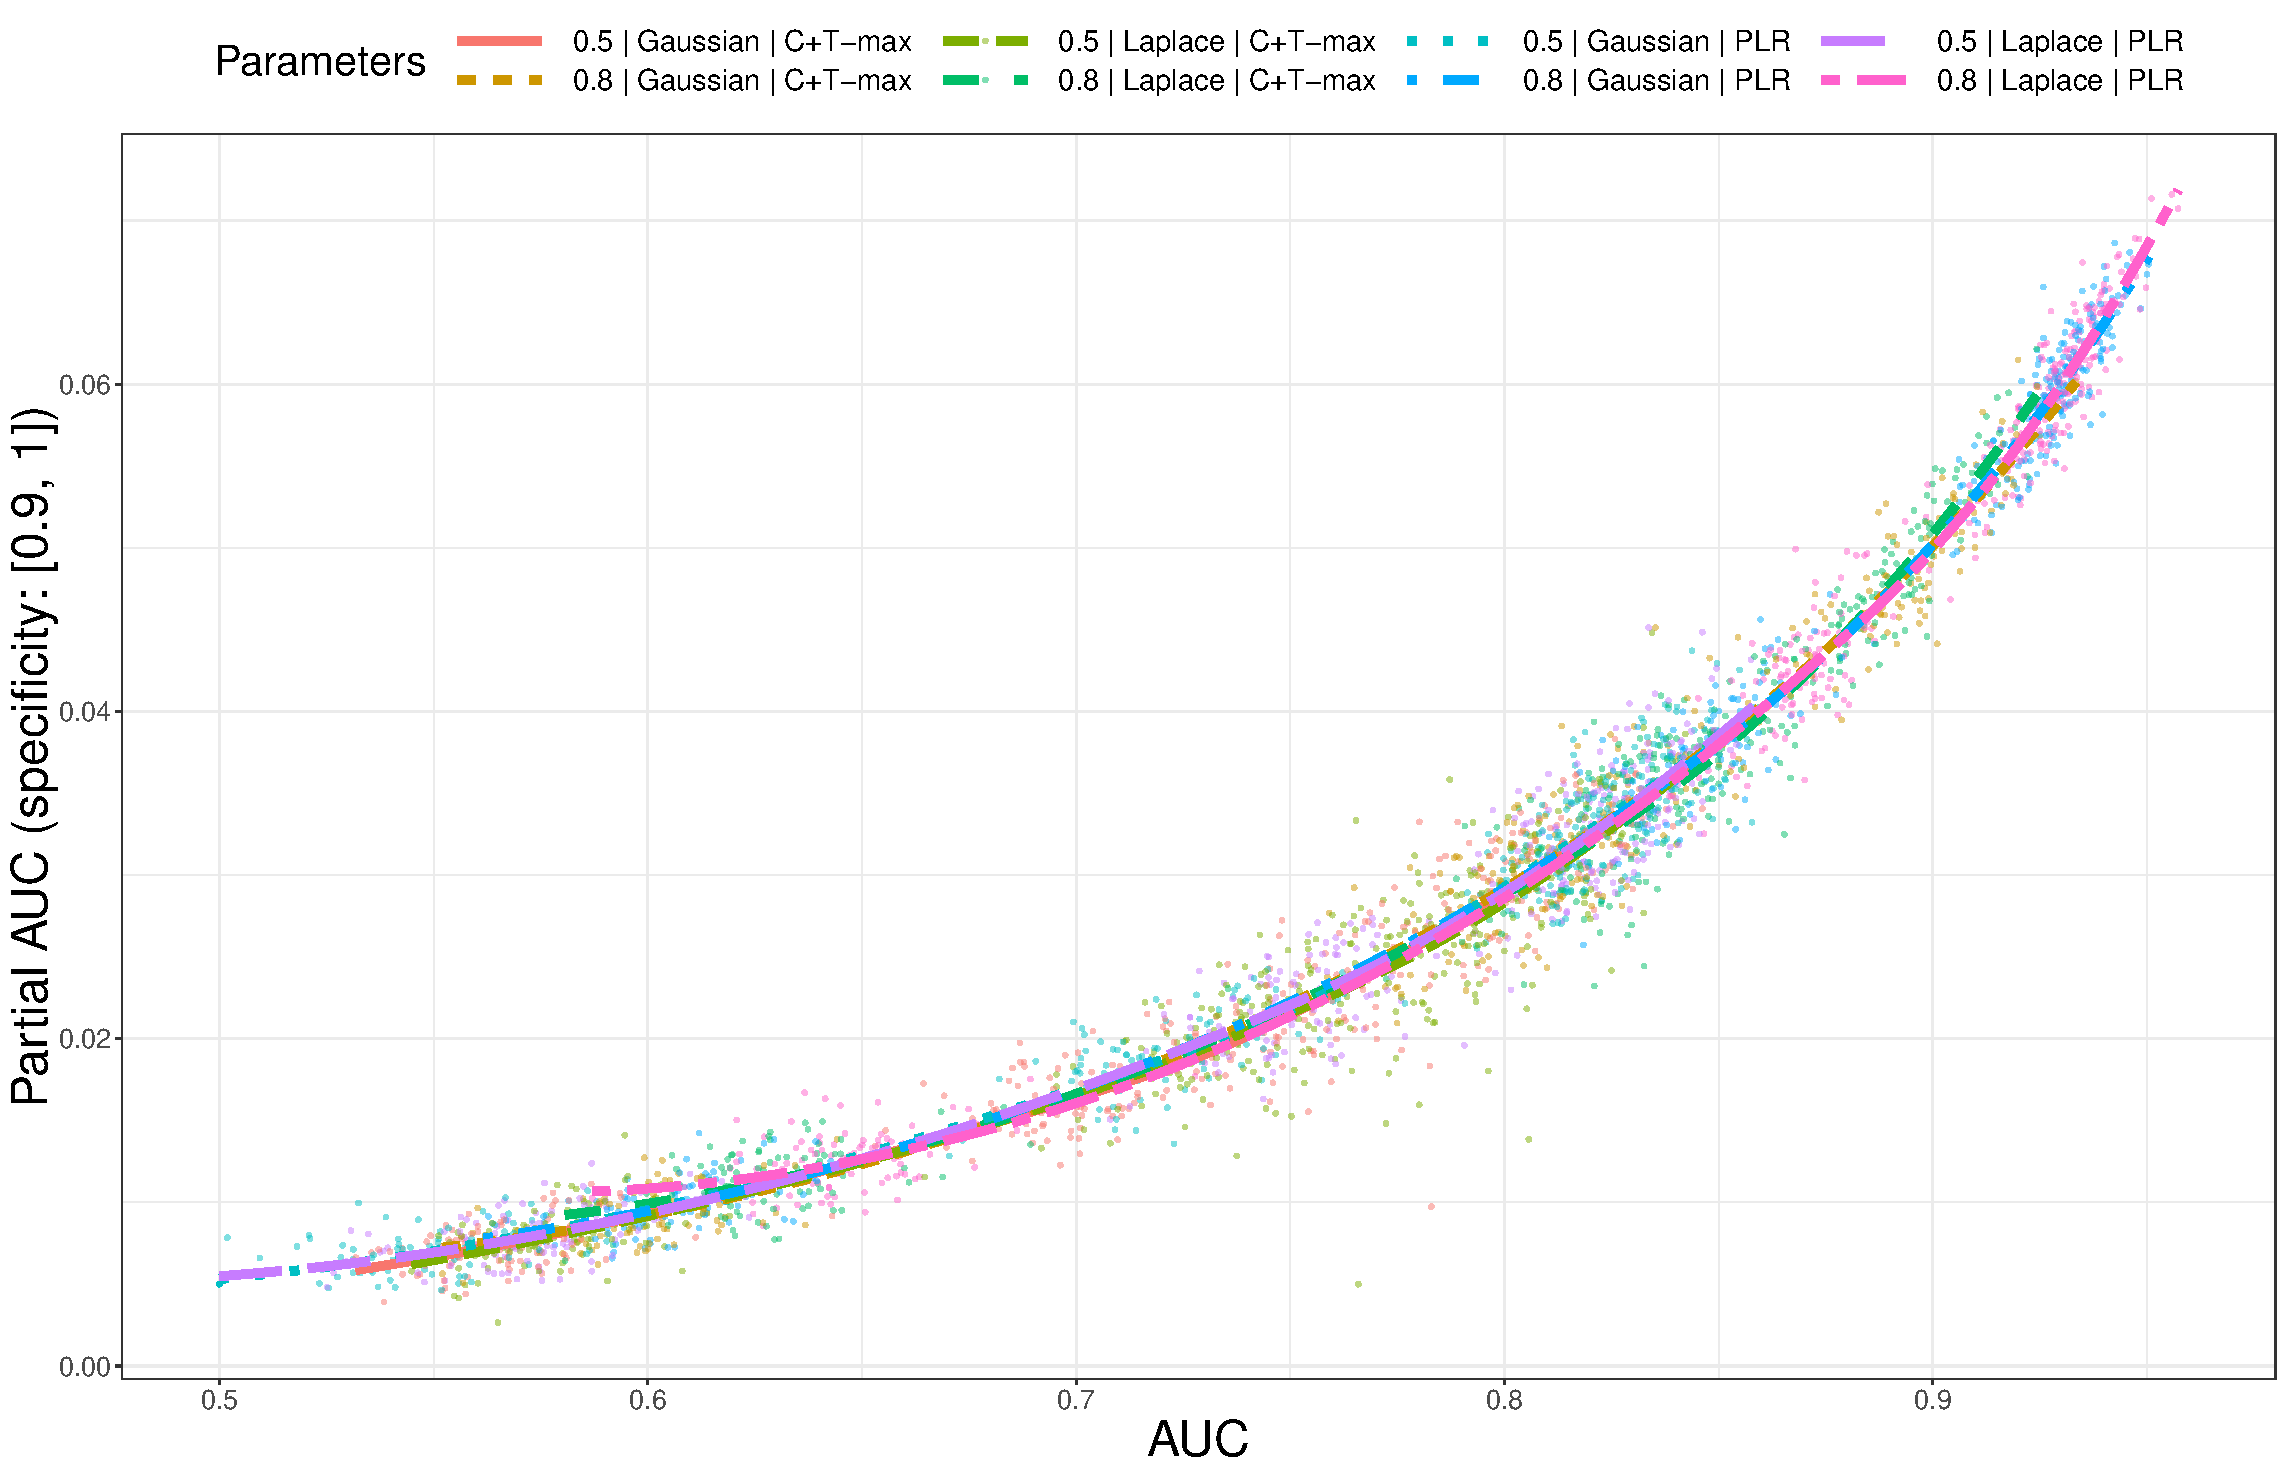
\includegraphics[width=\textwidth]{supp-AUC-corr}}
\caption{Scenario \textnumero1. Comparison of different predictive measures. ..There is a Spearman correlation.. of 98\% between values of AUC and partial AUC.[ADD]\label{fig:supp-AUC-corr}}
\end{figure}

%%%%%%%%%%%%%%%%%%%%%%%%%%%%%%%%%%%%%%%%%%%%%%%%%%%%%%%%%%%%%%%%%%%%%%%%%%%%%%%%

\newpage
\begin{figure}[h]
\centerline{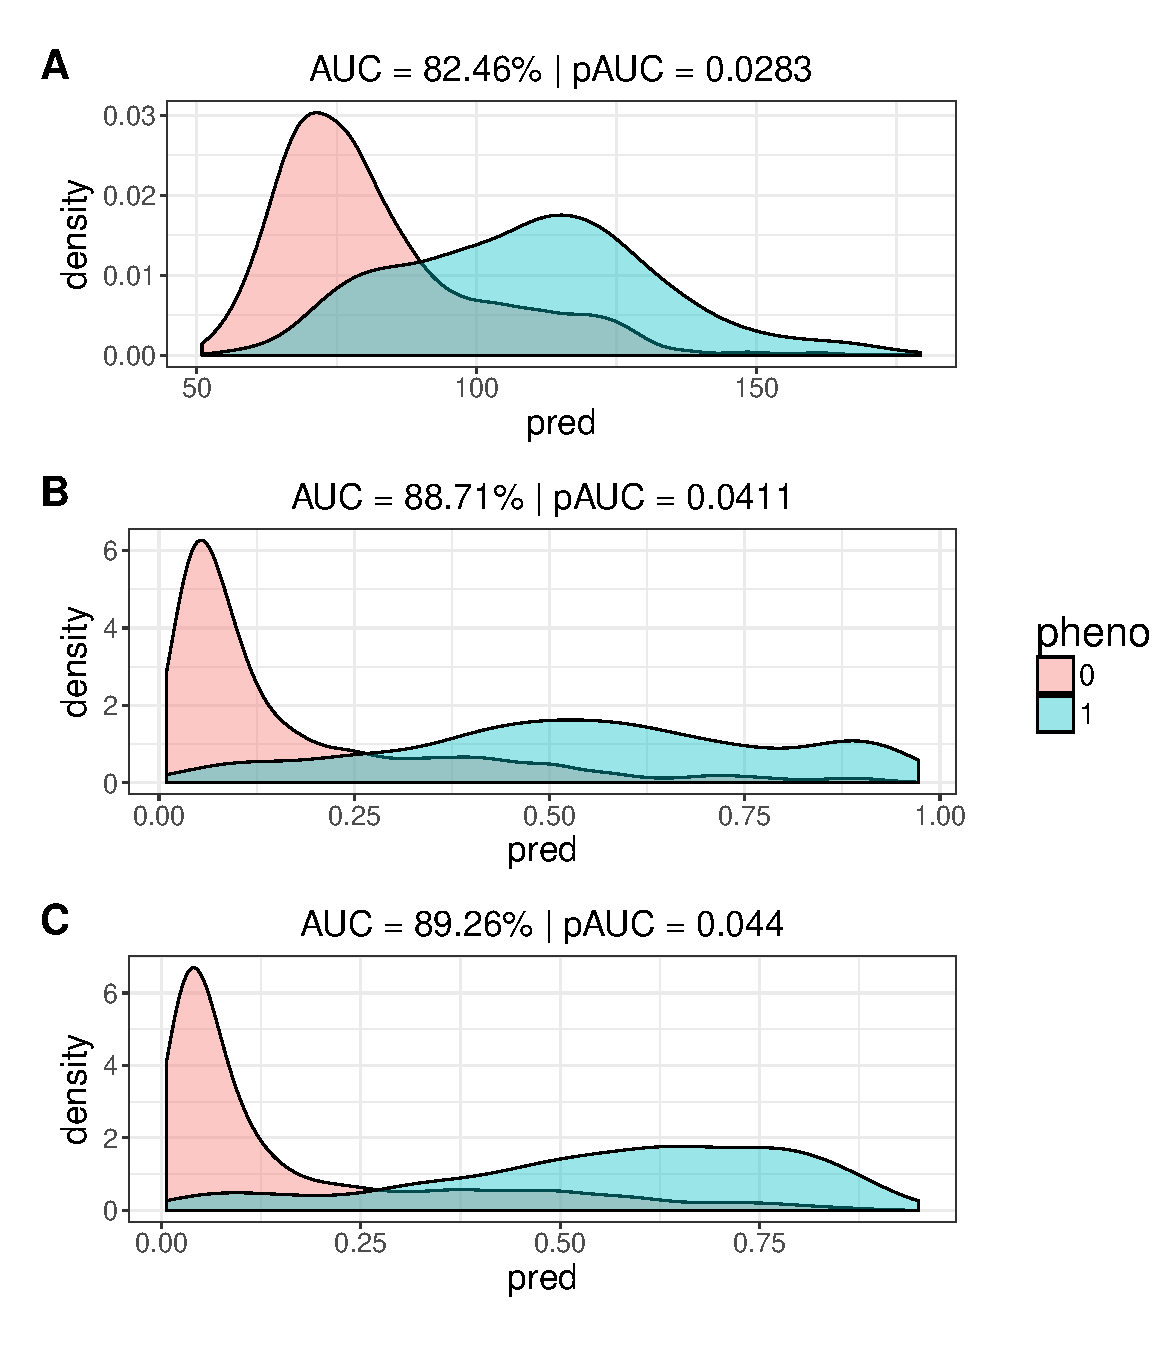
\includegraphics[width=\textwidth]{supp-score-densities}}
\caption{[ADD]\label{fig:supp-score-densities}}
\end{figure}

%%%%%%%%%%%%%%%%%%%%%%%%%%%%%%%%%%%%%%%%%%%%%%%%%%%%%%%%%%%%%%%%%%%%%%%%%%%%%%%%


\end{document}
